\documentclass[12pt, a4paper]{article}

% --- Packages ---
\usepackage[utf8]{inputenc}
\usepackage[T1]{fontenc}
\usepackage{geometry}
\geometry{a4paper, margin=1in, headheight=15pt}
\usepackage{xcolor}
\usepackage{hyperref}
\usepackage{graphicx}
\usepackage{tcolorbox}
\usepackage{fancyhdr}
\usepackage{titlesec}
\usepackage{enumitem}
\usepackage{parskip}
\usepackage{caption}
\usepackage{float}
\usepackage{listings}

% --- Colors ---
\definecolor{primary}{RGB}{12, 74, 110}     % Dark Slate Blue
\definecolor{secondary}{RGB}{2, 132, 199}   % Sky Blue
\definecolor{accent}{RGB}{240, 249, 255}    % Very Light Blue for backgrounds
\definecolor{darkgray}{RGB}{71, 85, 105}
\definecolor{codebg}{RGB}{248, 250, 252}

% --- Hyperref Setup ---
\hypersetup{
    colorlinks=true,
    linkcolor=primary,
    filecolor=secondary,      
    urlcolor=secondary,
    pdftitle={Comprehensive Week 5 Report - CalderR Internship},
    pdfpagemode=FullScreen,
}

% --- Header and Footer Setup ---
\pagestyle{fancy}
\fancyhf{}
\rhead{\textcolor{darkgray}{\textbf{Week 5 Comprehensive Report}}}
\lhead{\textcolor{darkgray}{CalderR Agentic AI Internship, 2026}}
\cfoot{\textcolor{darkgray}{Page \thepage}}
\renewcommand{\headrulewidth}{0.4pt}
\renewcommand{\footrulewidth}{0.4pt}

% --- Section Formatting ---
\titleformat{\section}
  {\LARGE\bfseries\color{primary}}{\thesection}{1em}{}[{\titlerule[1.2pt]}]

\titleformat{\subsection}
  {\Large\bfseries\color{secondary}}{\thesubsection}{1em}{}

\titleformat{\subsubsection}
  {\large\bfseries\color{primary}}{\thesubsubsection}{1em}{}

% --- Document Starts Here ---
\begin{document}

% --- Title Page ---
\begin{titlepage}
    \centering
    \vspace*{2cm}
    
    {\Huge \textbf{\textcolor{primary}{Agentic AI Engineering Internship}}} \\[0.5cm]
    {\Huge \textbf{\textcolor{primary}{2026}}} \\[1.5cm]
    
    {\LARGE \textbf{Week 5 Comprehensive Report}} \\[0.5cm]
    {\Large \textit{AI Fundamentals \& Agentic AI Foundations: \\ Multi-Agent Systems}} \\[2cm]
    
    \begin{tcolorbox}[colback=accent, colframe=primary, rounded corners, boxrule=1.5pt, width=0.75\textwidth, arc=4mm]
        \centering
        \vspace{0.4cm}
        {\Large \textbf{Prepared By:}} \\[0.2cm]
        {\Large \textbf{Ghafoor}} \\[0.4cm]
        {\large \textbf{Date:}} \\
        {\large \today}
        \vspace{0.4cm}
    \end{tcolorbox}
    
    \vfill
    
    {\huge \textbf{\textcolor{secondary}{CalderR.}}} \\[0.2cm]
    {\large \textit{RETHINKING $\cdot$ HOW $\cdot$ WORK $\cdot$ WORKS}}
    \vspace*{1cm}
\end{titlepage}

% --- Table of Contents ---
\tableofcontents
\newpage

% --- Section 1: Executive Summary ---
\section{Executive Summary}
This comprehensive report details the theoretical concepts, practical lab exercises, and ambitious multi-agent projects completed during Week 5 of the CalderR Agentic AI Engineering Internship. Transitioning from single-agent systems to coordinated teams, the focus of the week was orchestrating teams of AI agents to solve complex problems collaboratively. 

The week emphasized advanced architectures including orchestrator-worker, supervisor patterns, and hierarchical teams. By engineering structured agent-to-agent communication via typed message passing and implementing robust conflict resolution and failure handling mechanisms, the foundation for highly resilient production-ready multi-agent systems was established.

The culmination of these learnings is showcased in two sophisticated projects: the \textbf{Autonomous Competitive Intelligence Agent} (Intermediate) and the \textbf{Autonomous AI Research Lab} (Production). These solutions demonstrate true parallel agent execution, confidence-weighted consensus, dynamic agent assembly, and explicit observability.

% --- Section 2: Conceptual Mastery & Assessment ---
\section{Conceptual Mastery \& Assessment}
The curriculum this week demanded a deep dive into the architectural principles and operational patterns that govern effective multi-agent collaboration.

\subsection{Multi-Agent Architectures \& Communication}
\begin{itemize}[label=\textcolor{secondary}{$\bullet$}]
    \item \textbf{Architectural Patterns:} Mastered orchestrator-worker models, supervisor chains, peer networks, and hierarchical teams. Identified when a single agent outperforms a team versus when task delegation is crucial.
    \item \textbf{Typed Message Passing:} Replaced raw strings with structured Pydantic schemas (TaskRequest, TaskResult, ErrorReport, Handoff) for inter-agent communication, drastically improving reliability and type safety.
    \item \textbf{Specialization Design:} Engineered specialized agent personas with distinct tooling, authority scopes, and domain expertise.
    \item \textbf{Failure Handling \& Consensus:} Implemented resilient supervisor logic that gracefully handles timeouts and low-confidence responses through retry or fallback routing. Engineered debate patterns and confidence-weighted consensus to adjudicate contradictions explicitly.
    \item \textbf{Observability:} Instrumenting systems with per-agent logging for token usage, latency, and decision tracking via LangSmith and structured audit trails.
\end{itemize}

\newpage

% --- Section 3: Production Project ---
\section{Production Project: Autonomous AI Research Lab}

\begin{tcolorbox}[colback=accent, colframe=primary, title=\textbf{Architectural Overview}, boxrule=1pt]
A fully autonomous research system that takes a natural-language research question, dynamically assembles a team of specialist agents based on the domain, executes a multi-phase research process (hypothesis, evidence gathering, critic, synthesis, peer review), and publishes a professional report without human intervention.
\end{tcolorbox}

\begin{figure}[H]
    \centering
    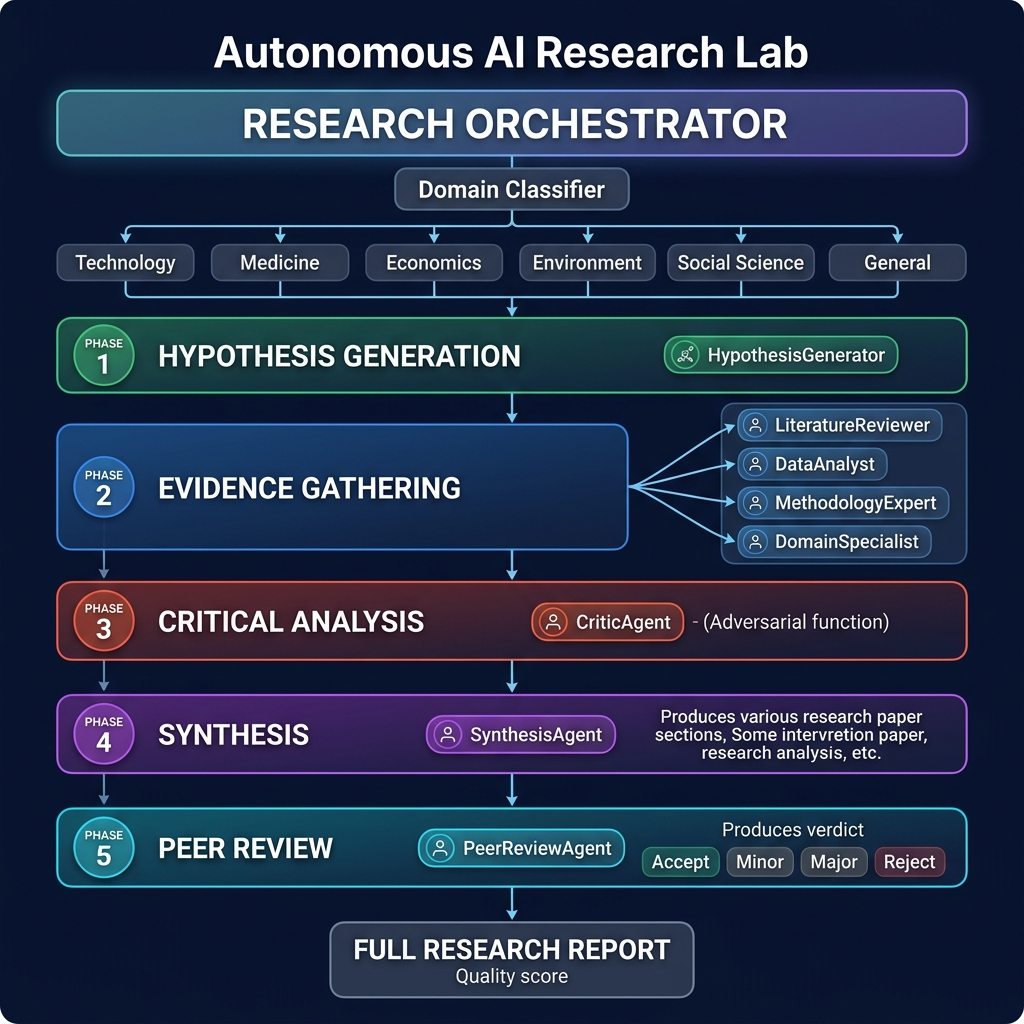
\includegraphics[width=0.85\textwidth]{projects/research_lab/architecture.png}
    \caption{Production Project: Autonomous AI Research Lab Architecture}
\end{figure}

\subsection{Technical Implementation}
\begin{itemize}[label=\textcolor{secondary}{$\bullet$}]
    \item \textbf{Dynamic Agent Assembly:} The Domain Classifier dynamically selects and instantiates 3--5 specialized Evidence Agents tailored to the research topic.
    \item \textbf{Multi-Phase Orchestration:} Utilized LangGraph subgraphs to manage a hierarchical flow: hypothesis generation $\rightarrow$ parallel evidence gathering $\rightarrow$ critical review $\rightarrow$ synthesis $\rightarrow$ peer review.
    \item \textbf{Critic \& Peer Review Patterns:} Implemented a Critic Agent to explicitly challenge weak links in evidence, and a Peer Review Agent to act as a second-pass quality check before publication.
    \item \textbf{Comprehensive Observability:} Features a FastAPI REST API, a Streamlit UI demonstrating real-time phase progress, and comprehensive LangSmith tracing for auditing decisions.
\end{itemize}

\subsection{System Demonstrations}
\begin{figure}[H]
    \centering
    \begin{minipage}{0.48\textwidth}
        \centering
        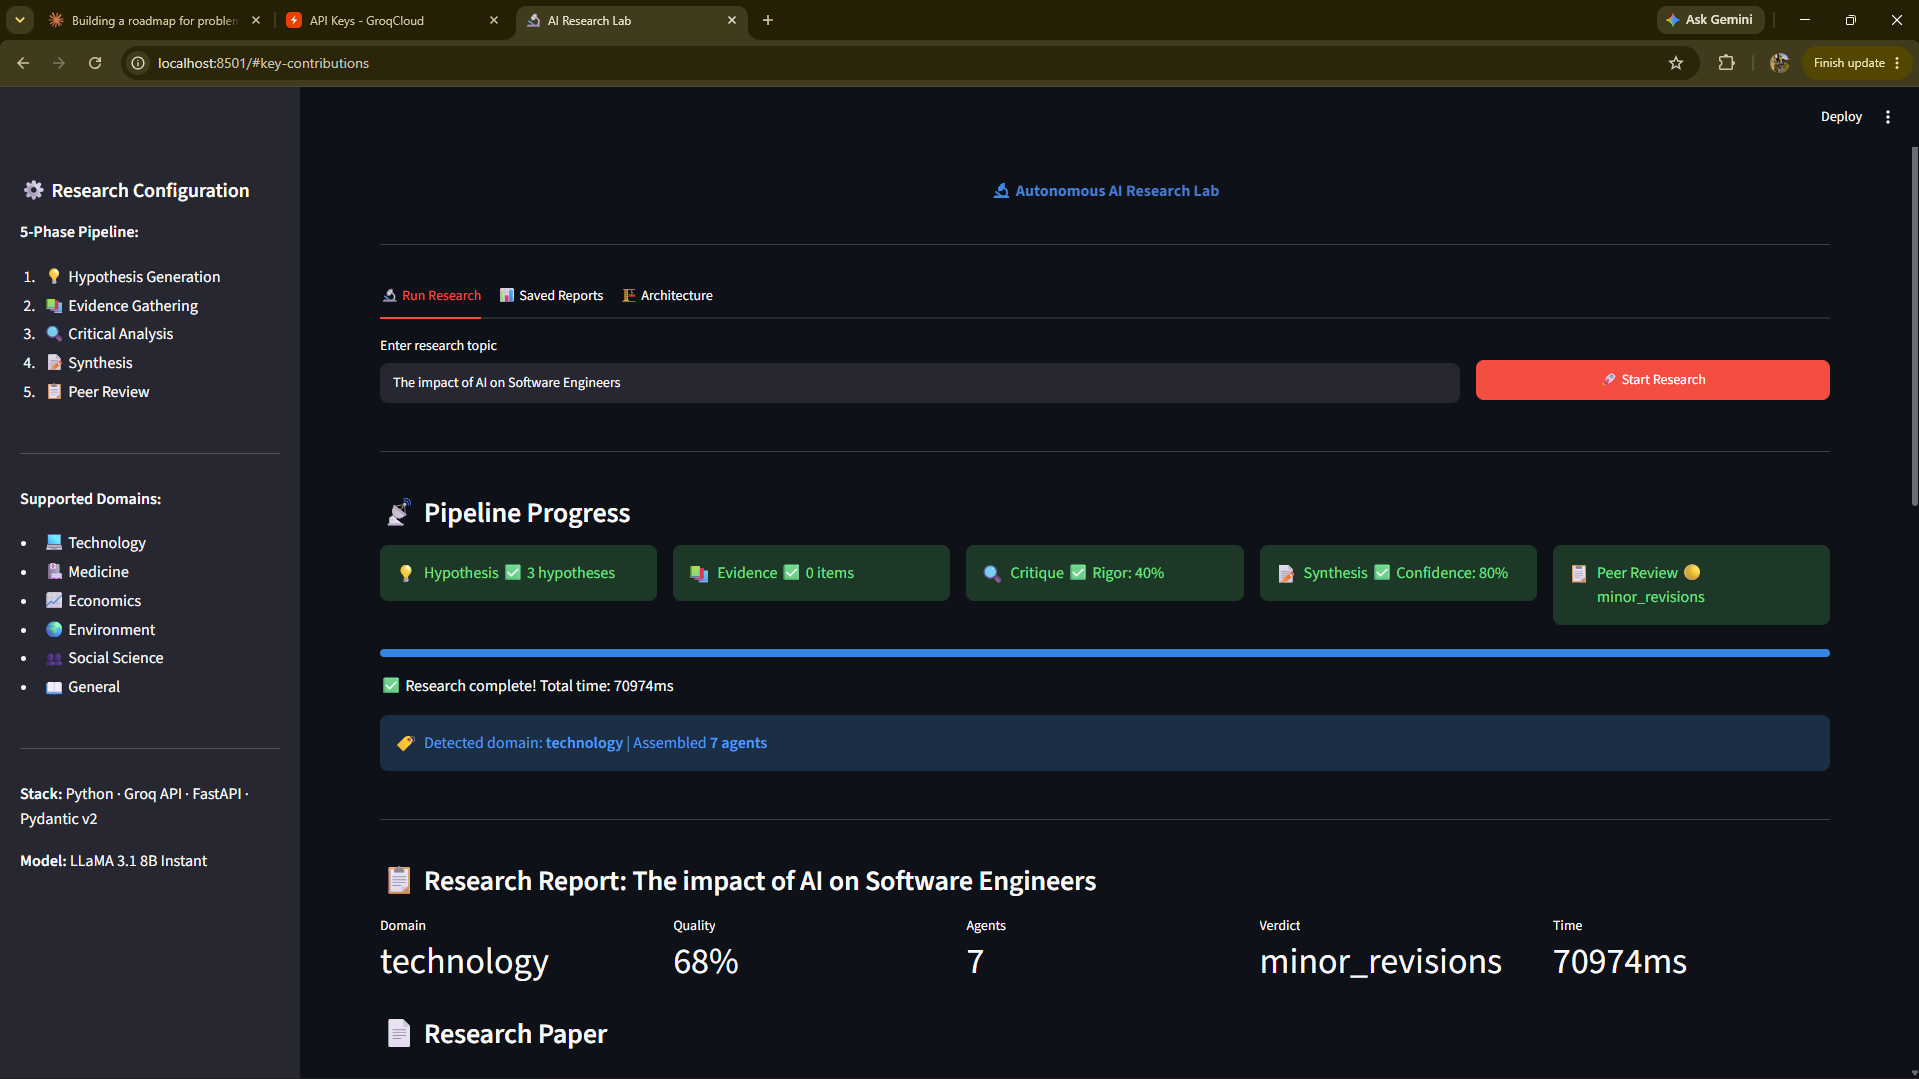
\includegraphics[width=\linewidth, keepaspectratio]{screenshots/Week5/Prod-1.png}
        \caption{Research Domain Classification}
    \end{minipage}\hfill
    \begin{minipage}{0.48\textwidth}
        \centering
        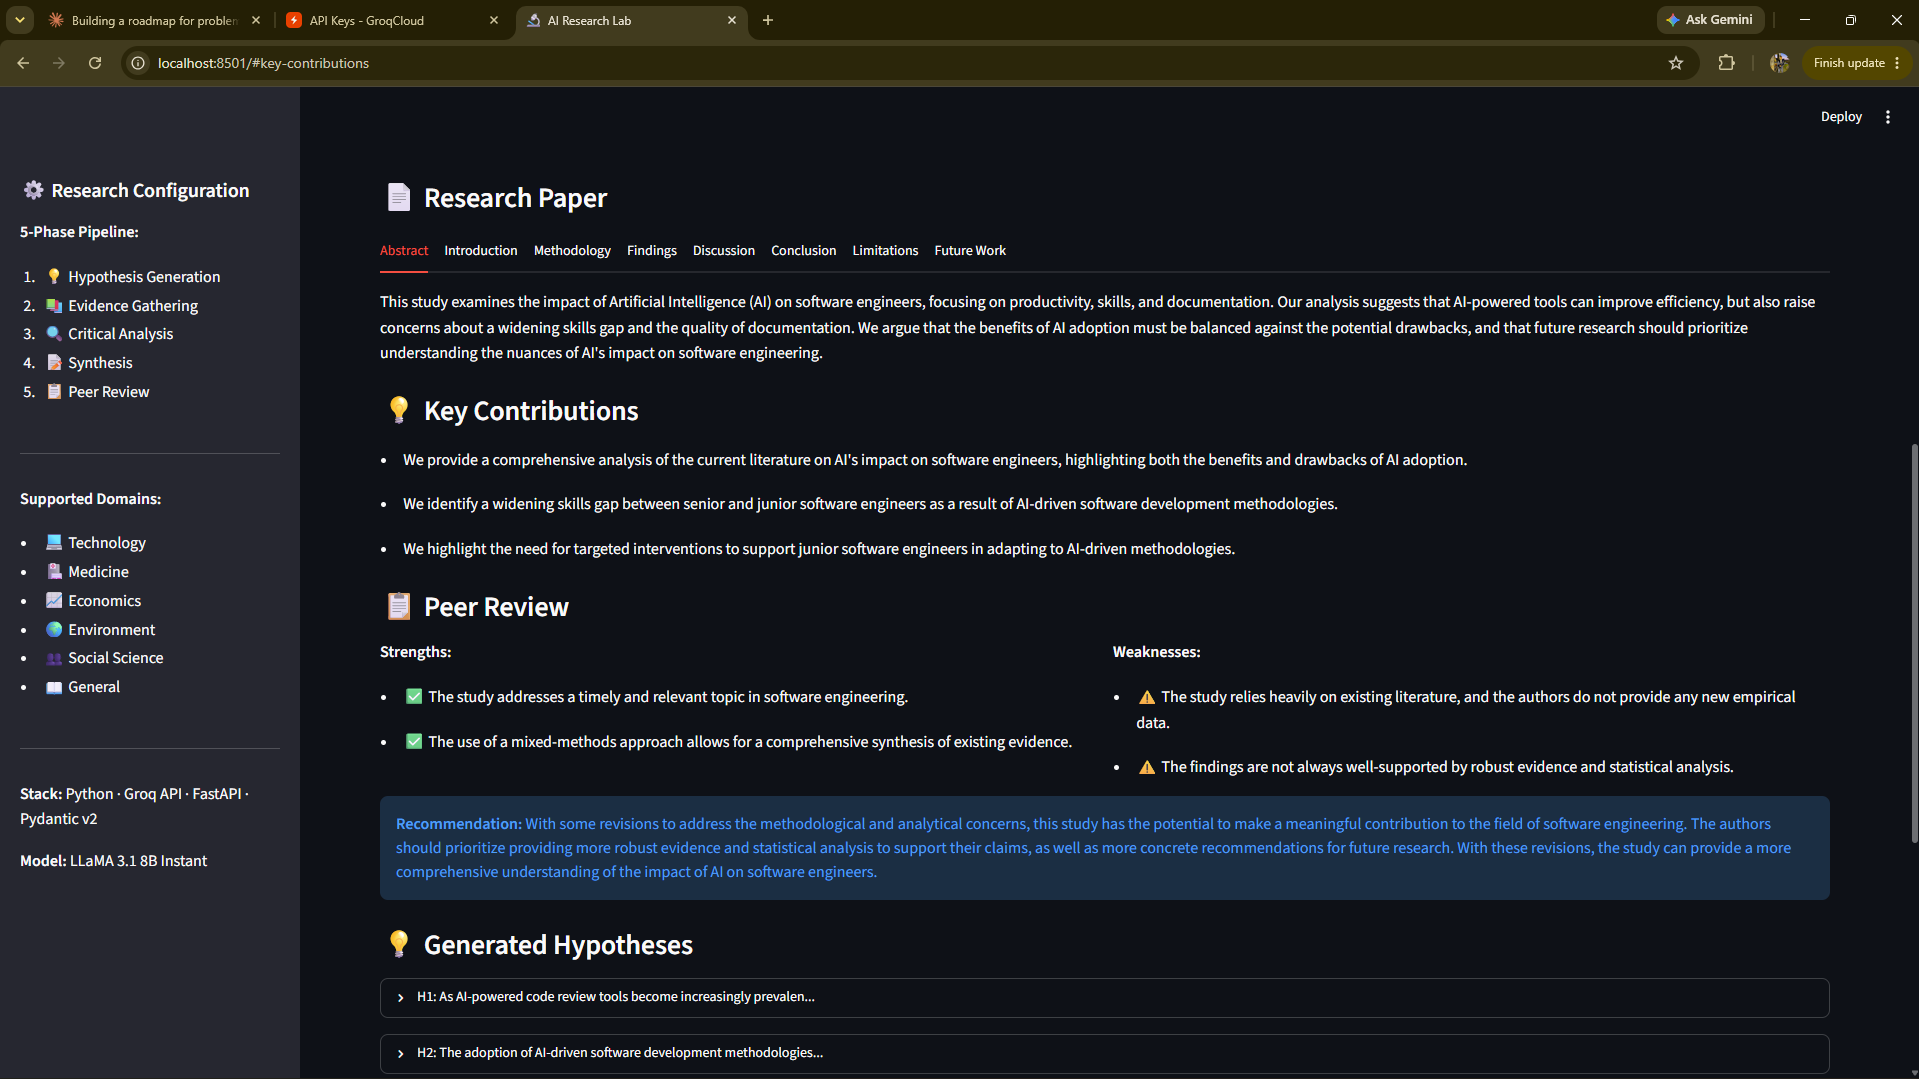
\includegraphics[width=\linewidth, keepaspectratio]{screenshots/Week5/Prod-2.png}
        \caption{Dynamic Agent Assembly}
    \end{minipage}
\end{figure}

\begin{figure}[H]
    \centering
    \begin{minipage}{0.48\textwidth}
        \centering
        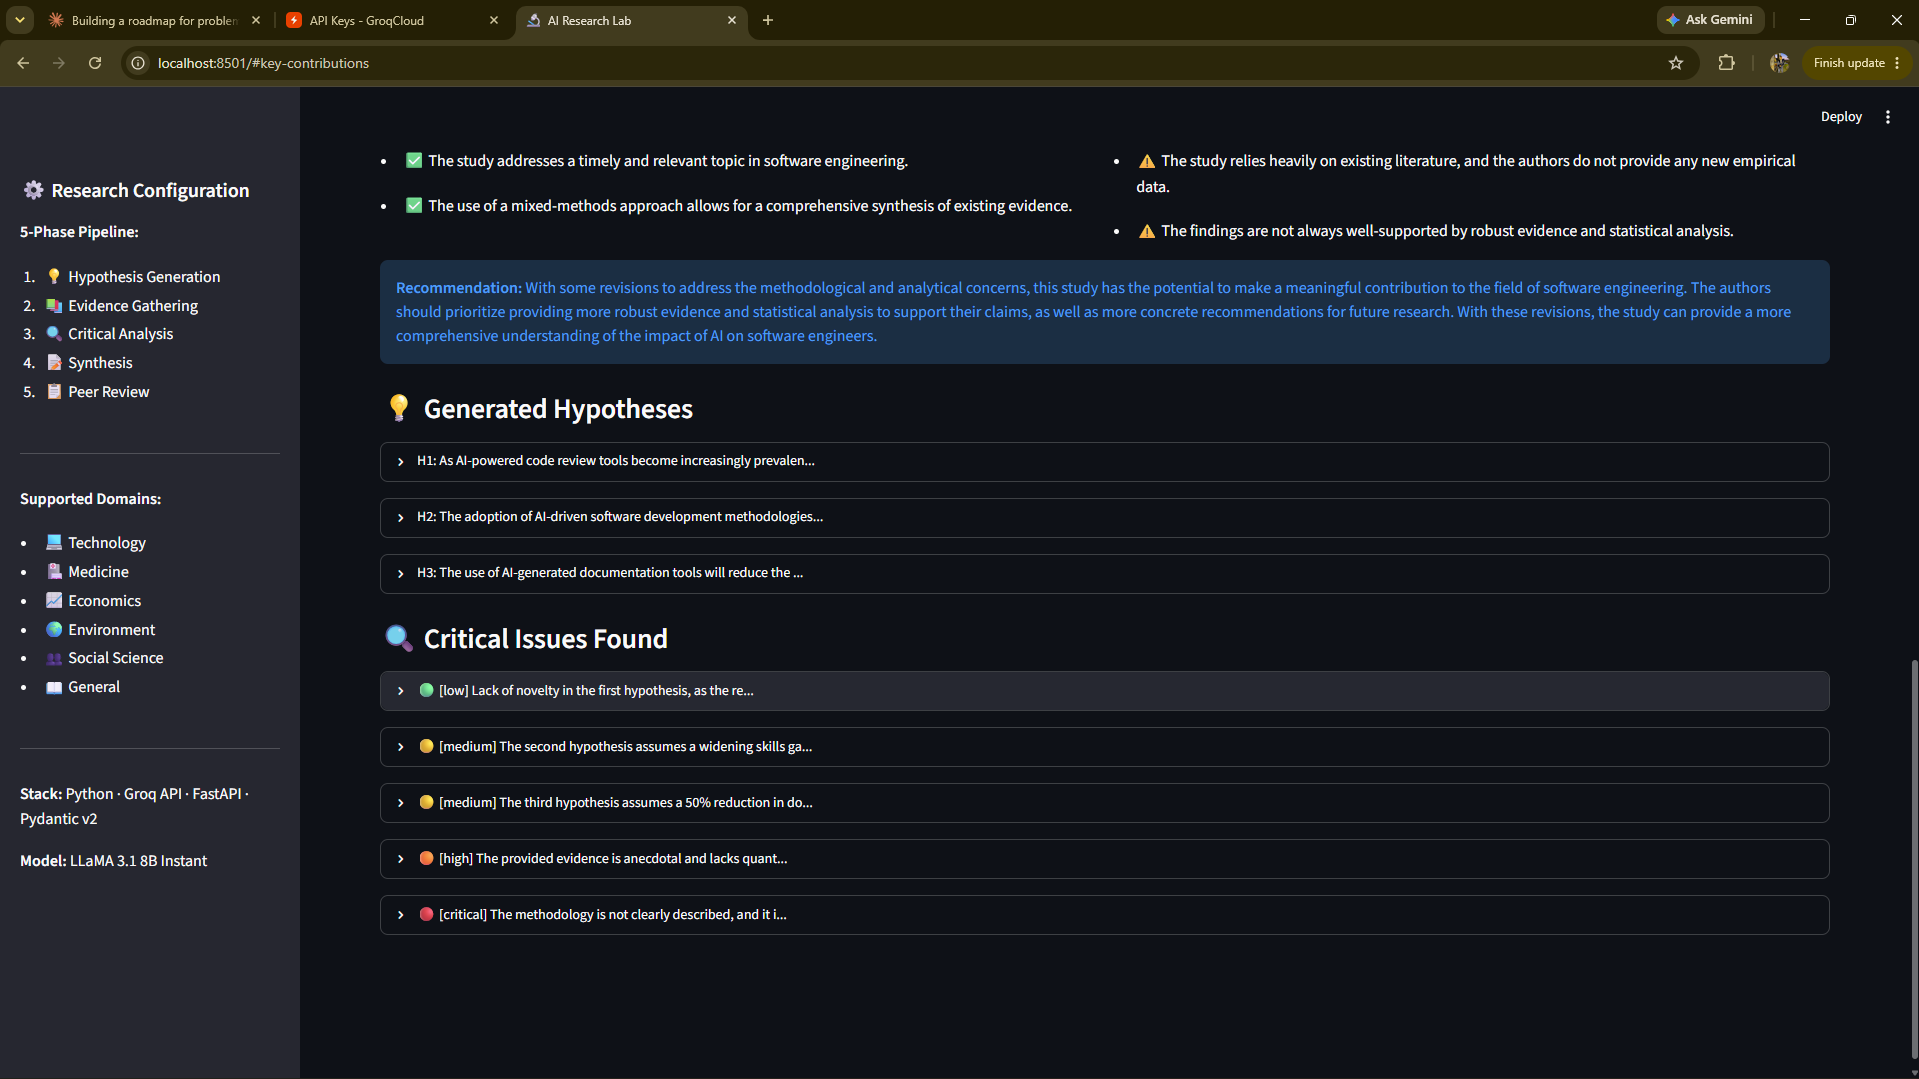
\includegraphics[width=\linewidth, keepaspectratio]{screenshots/Week5/Prod-3.png}
        \caption{RAG Evidence Gathering}
    \end{minipage}\hfill
    \begin{minipage}{0.48\textwidth}
        \centering
        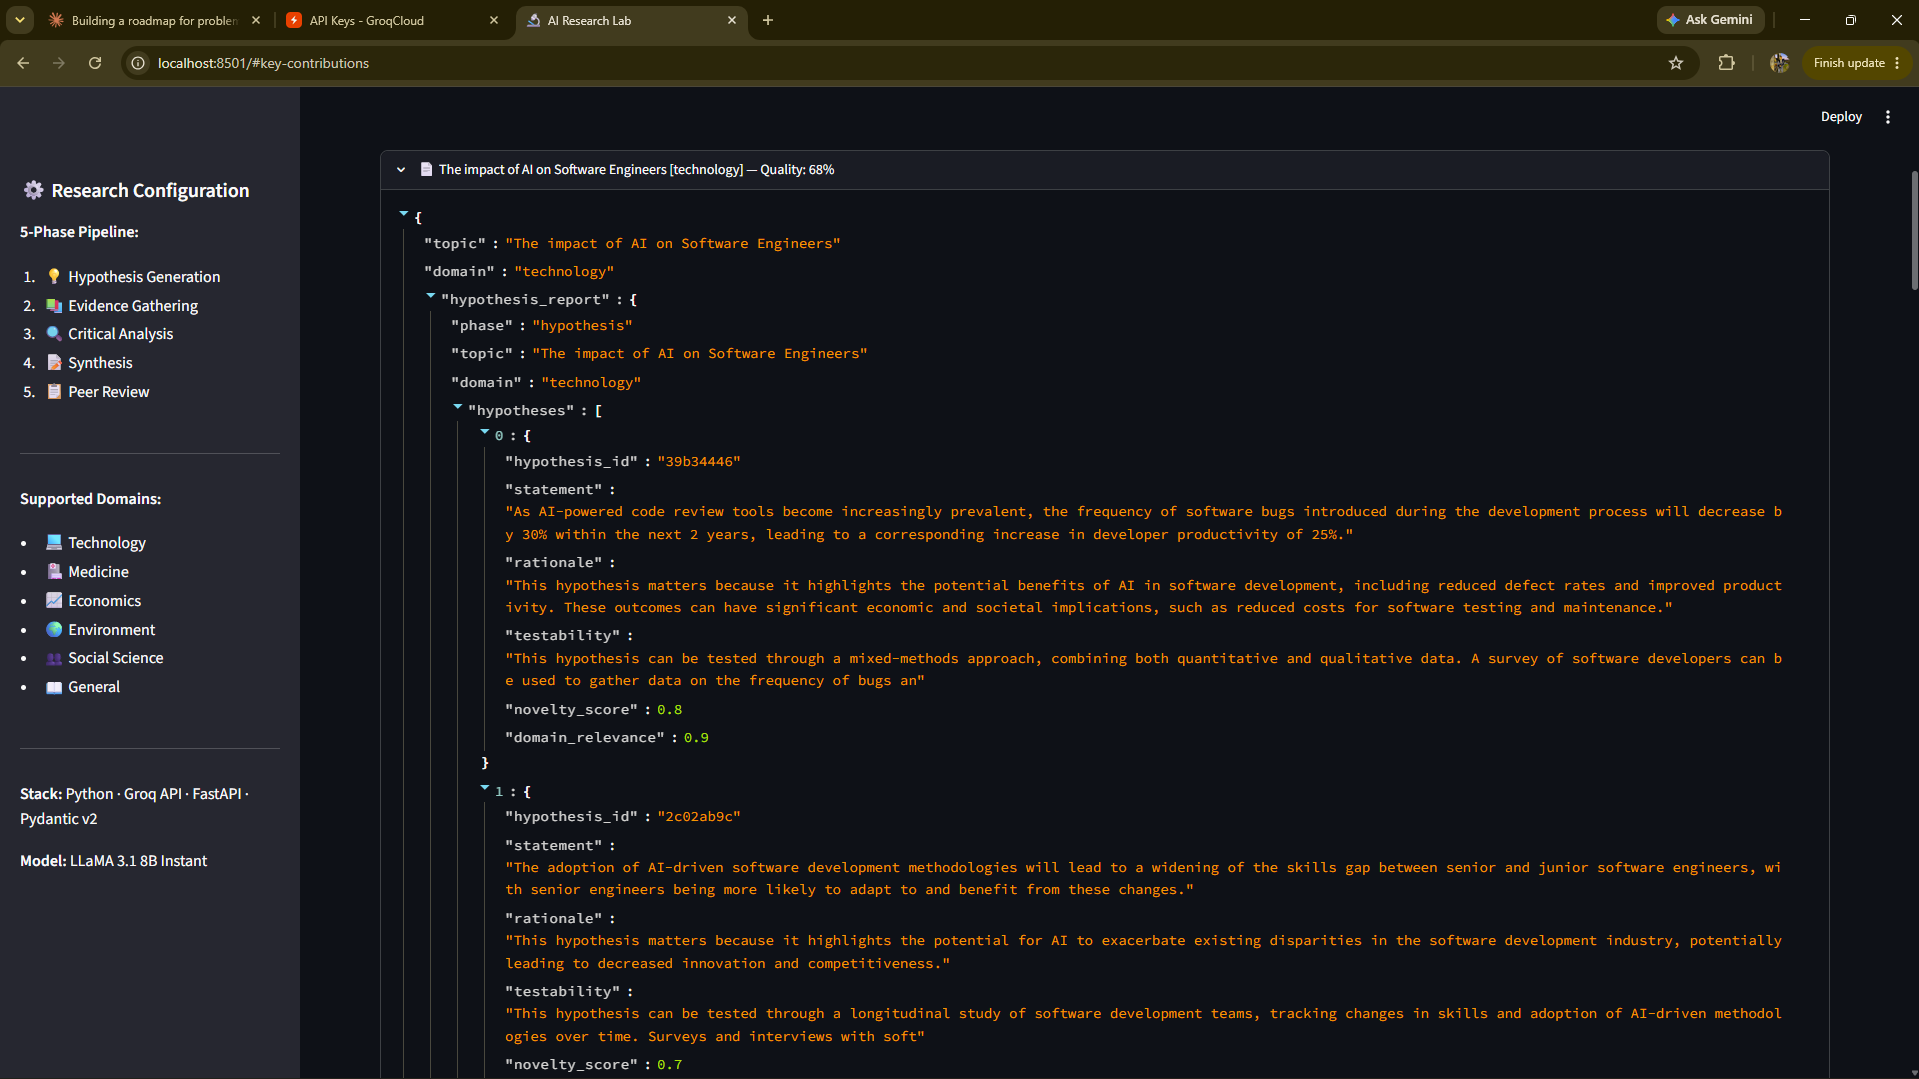
\includegraphics[width=\linewidth, keepaspectratio]{screenshots/Week5/Prod-4.png}
        \caption{Final Published Research Report}
    \end{minipage}
\end{figure}

\begin{figure}[H]
    \centering
    \begin{minipage}{0.48\textwidth}
        \centering
        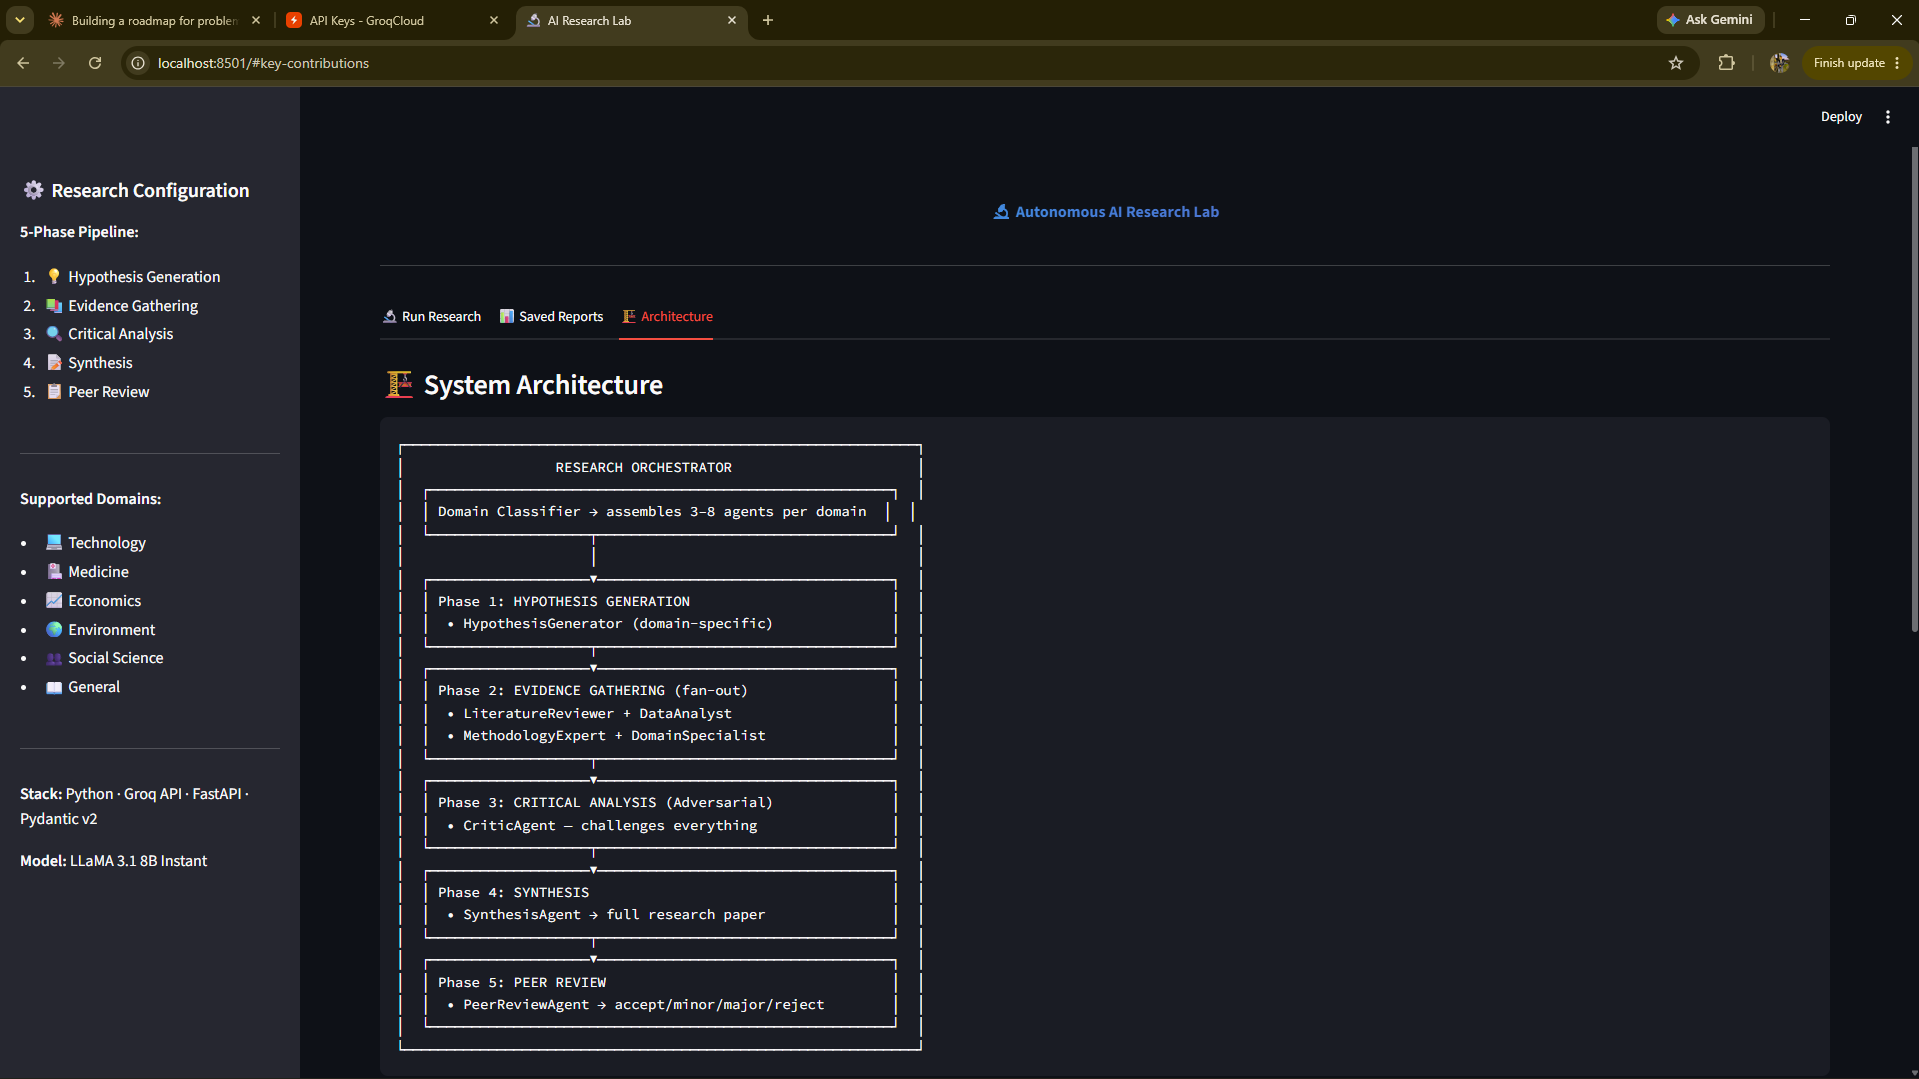
\includegraphics[width=\linewidth, keepaspectratio]{screenshots/Week5/Prod-5.png}
        \caption{System Architecture Diagram}
    \end{minipage}\hfill
    \begin{minipage}{0.48\textwidth}
        \centering
        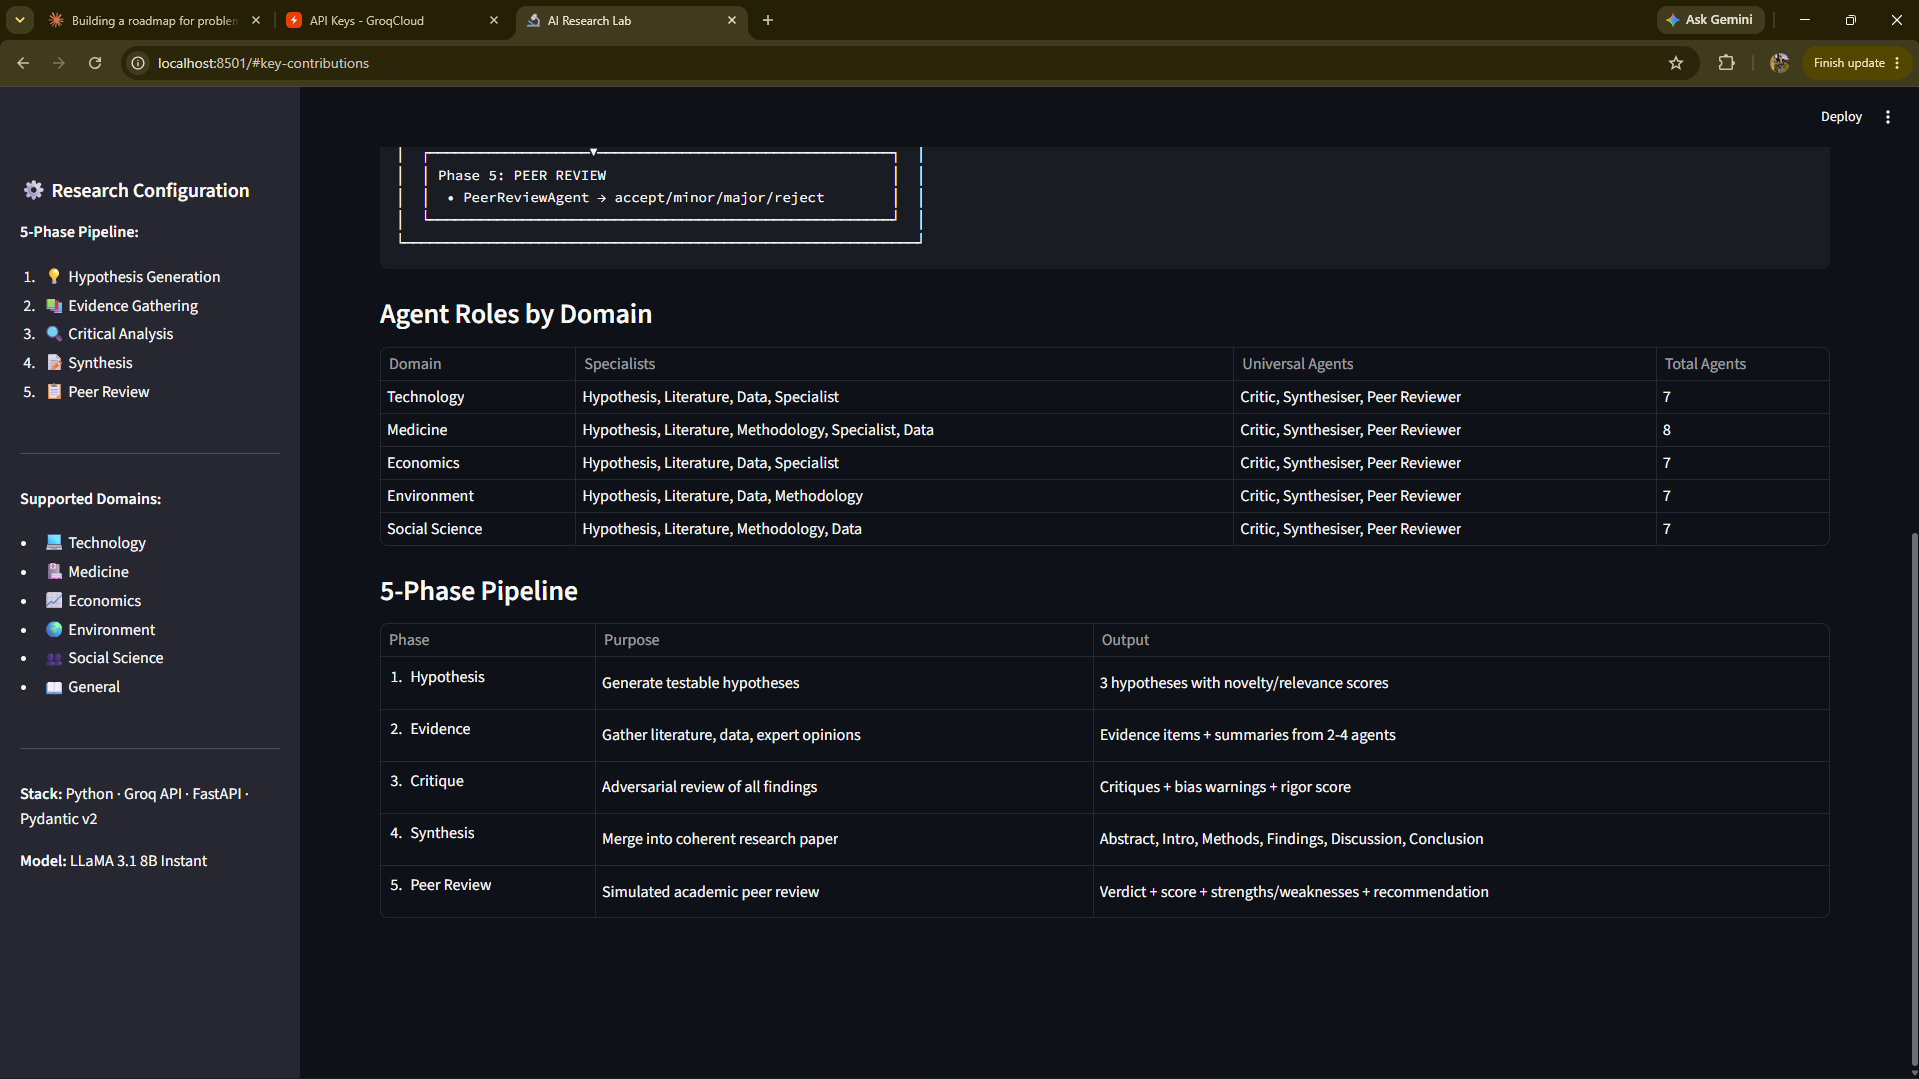
\includegraphics[width=\linewidth, keepaspectratio]{screenshots/Week5/Prod-6.png}
        \caption{Agent Roles \& Pipeline}
    \end{minipage}
\end{figure}

\newpage

% --- Section 4: Intermediate Project ---
\section{Intermediate Project: Autonomous Competitive Intelligence Agent}

\begin{tcolorbox}[colback=accent, colframe=primary, title=\textbf{Architectural Overview}, boxrule=1pt]
A multi-agent system designed to autonomously research a company from multiple angles (market, product, tech stack, news, sentiment). It utilizes parallel fan-out execution, incorporates conflict resolution logic, and aggregates findings into a structured, professional intelligence briefing.
\end{tcolorbox}

\begin{figure}[H]
    \centering
    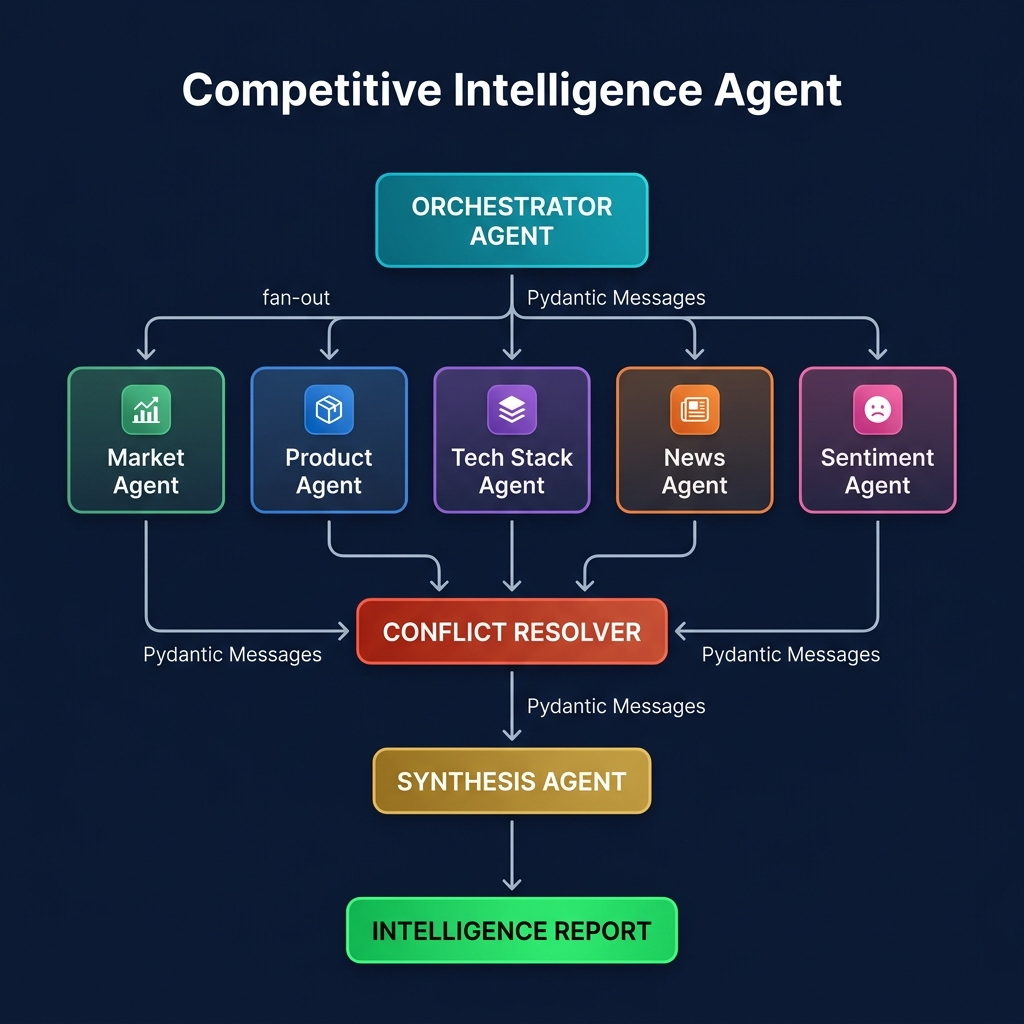
\includegraphics[width=0.85\textwidth]{projects/competitive_intel/architecture.png}
    \caption{Intermediate Project: Competitive Intelligence System Architecture}
\end{figure}

\subsection{Technical Implementation}
\begin{itemize}[label=\textcolor{secondary}{$\bullet$}]
    \item \textbf{Parallel Fan-Out Execution:} The Orchestrator Agent decomposes the research strategy and concurrently dispatches tasks to five specialized agents (Market, Product, Tech Stack, News, Sentiment).
    \item \textbf{Conflict Adjudication:} Embedded a Conflict Resolver agent that detects and adjudicates contradictions between individual agent findings before final synthesis.
    \item \textbf{Structured Typed Outputs:} Ensured every agent strictly adheres to Pydantic schemas, enabling reliable aggregation and generation of a clean, non-redundant Markdown report exposed via FastAPI and Streamlit.
\end{itemize}

\subsection{System Demonstrations}
\begin{figure}[H]
    \centering
    \begin{minipage}{0.48\textwidth}
        \centering
        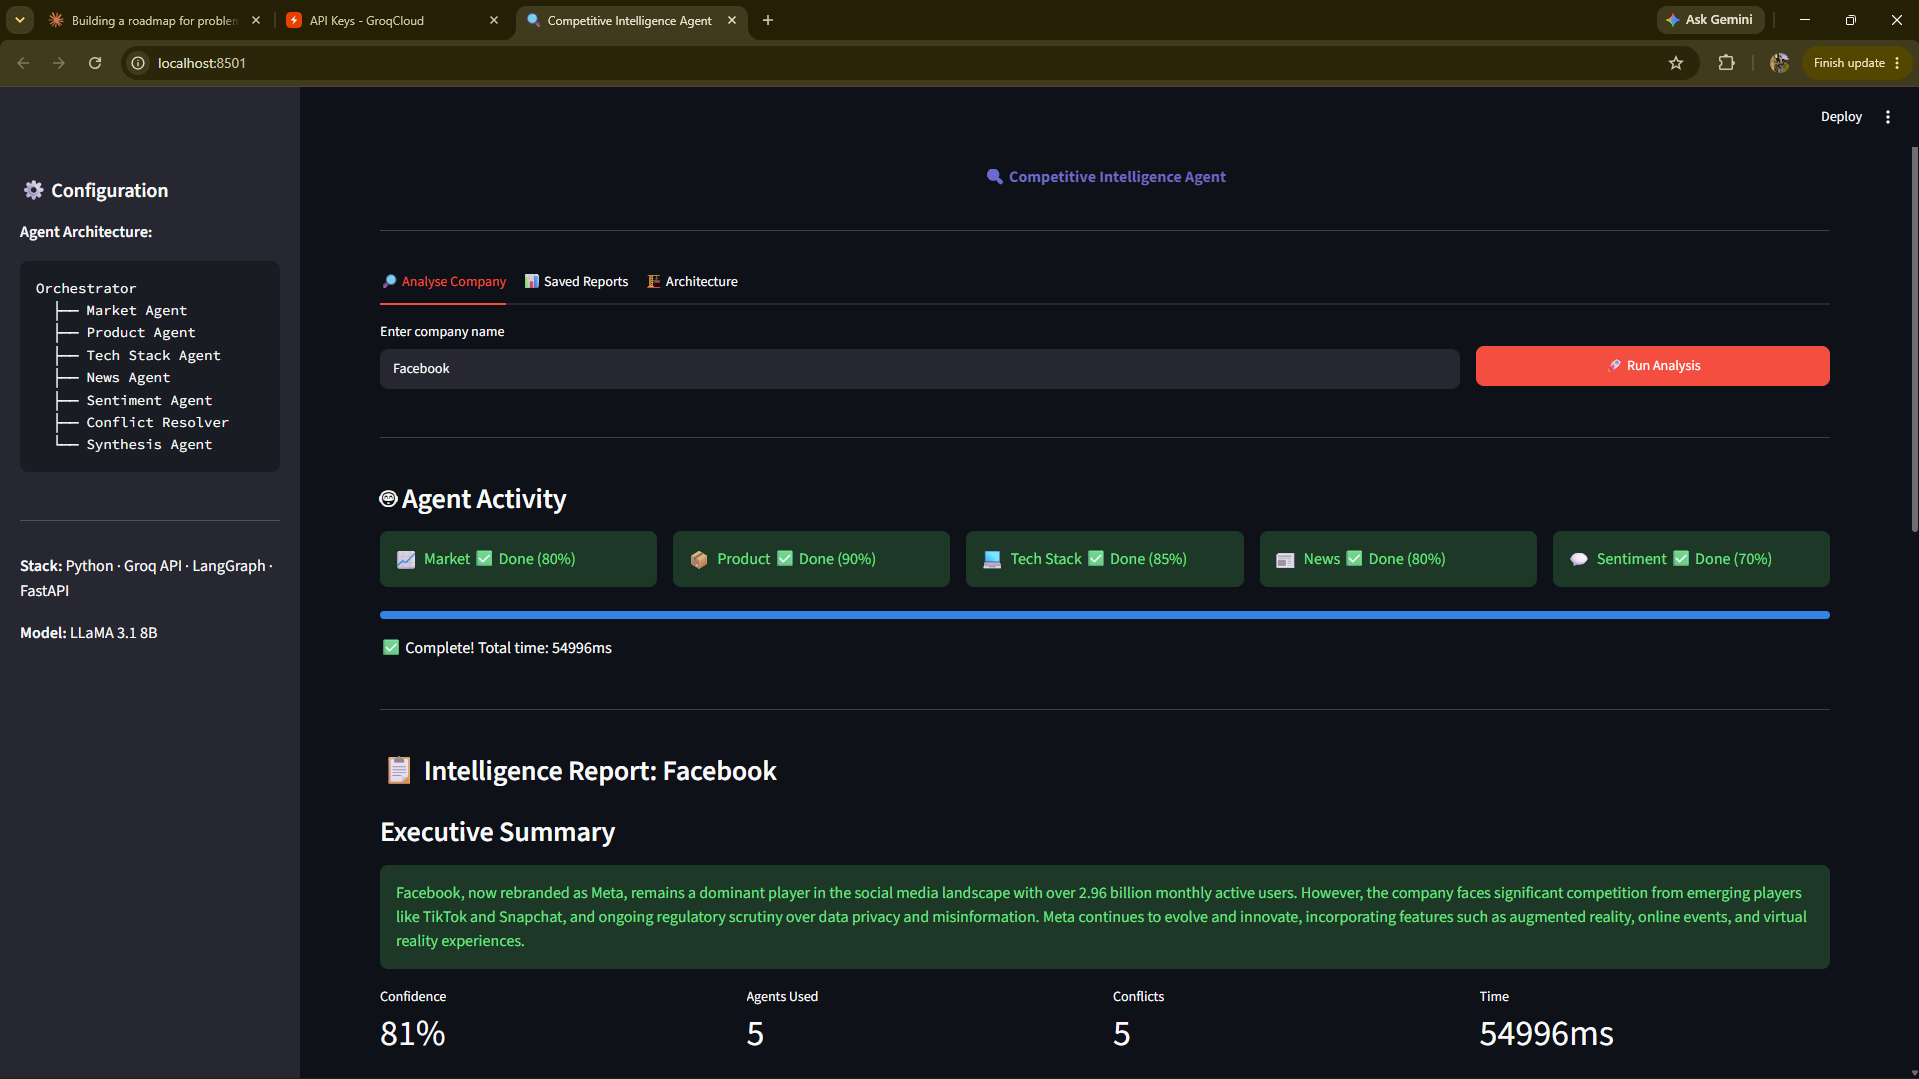
\includegraphics[width=\linewidth, keepaspectratio]{screenshots/Week5/Inter-1.png}
        \caption{Parallel Dispatch \& Agent Activity}
    \end{minipage}\hfill
    \begin{minipage}{0.48\textwidth}
        \centering
        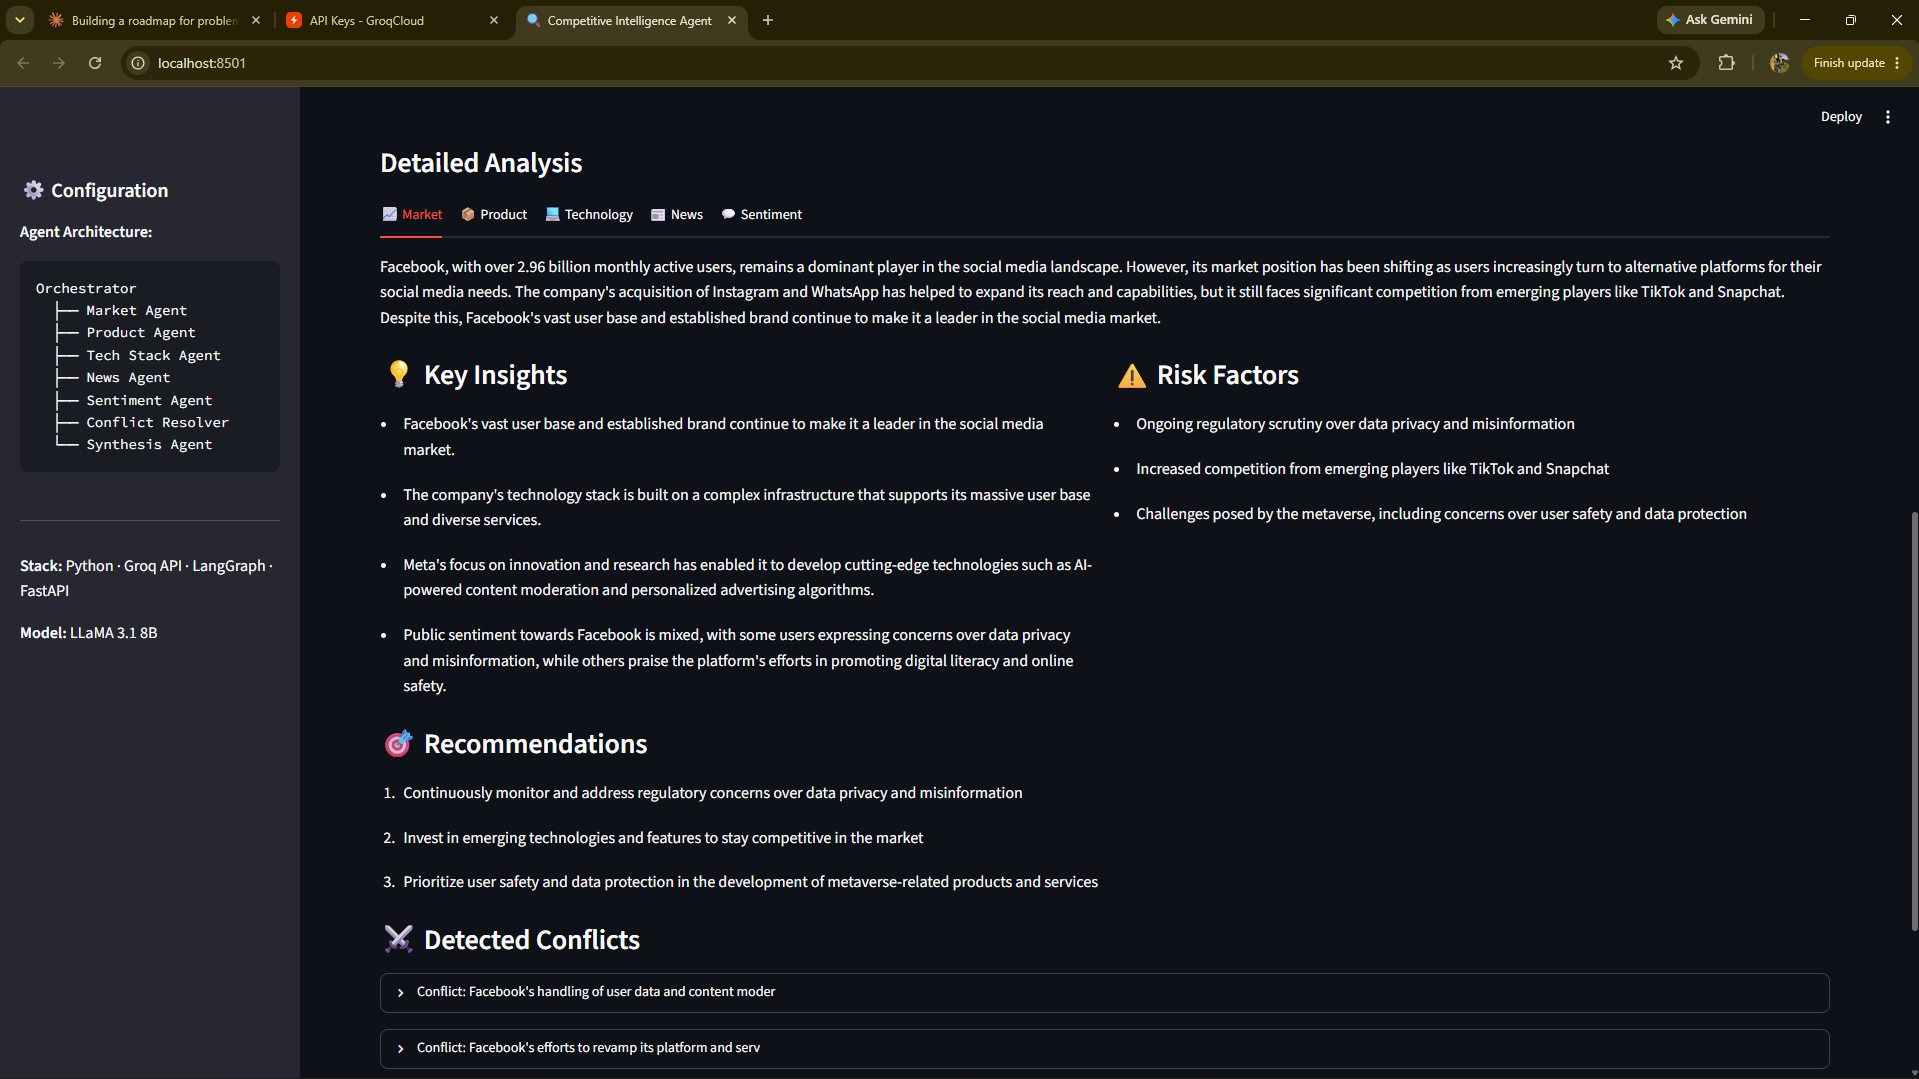
\includegraphics[width=\linewidth, keepaspectratio]{screenshots/Week5/Inter-2.png}
        \caption{Conflict Resolution Log \& Detailed Analysis}
    \end{minipage}
\end{figure}

\begin{figure}[H]
    \centering
    \begin{minipage}{0.48\textwidth}
        \centering
        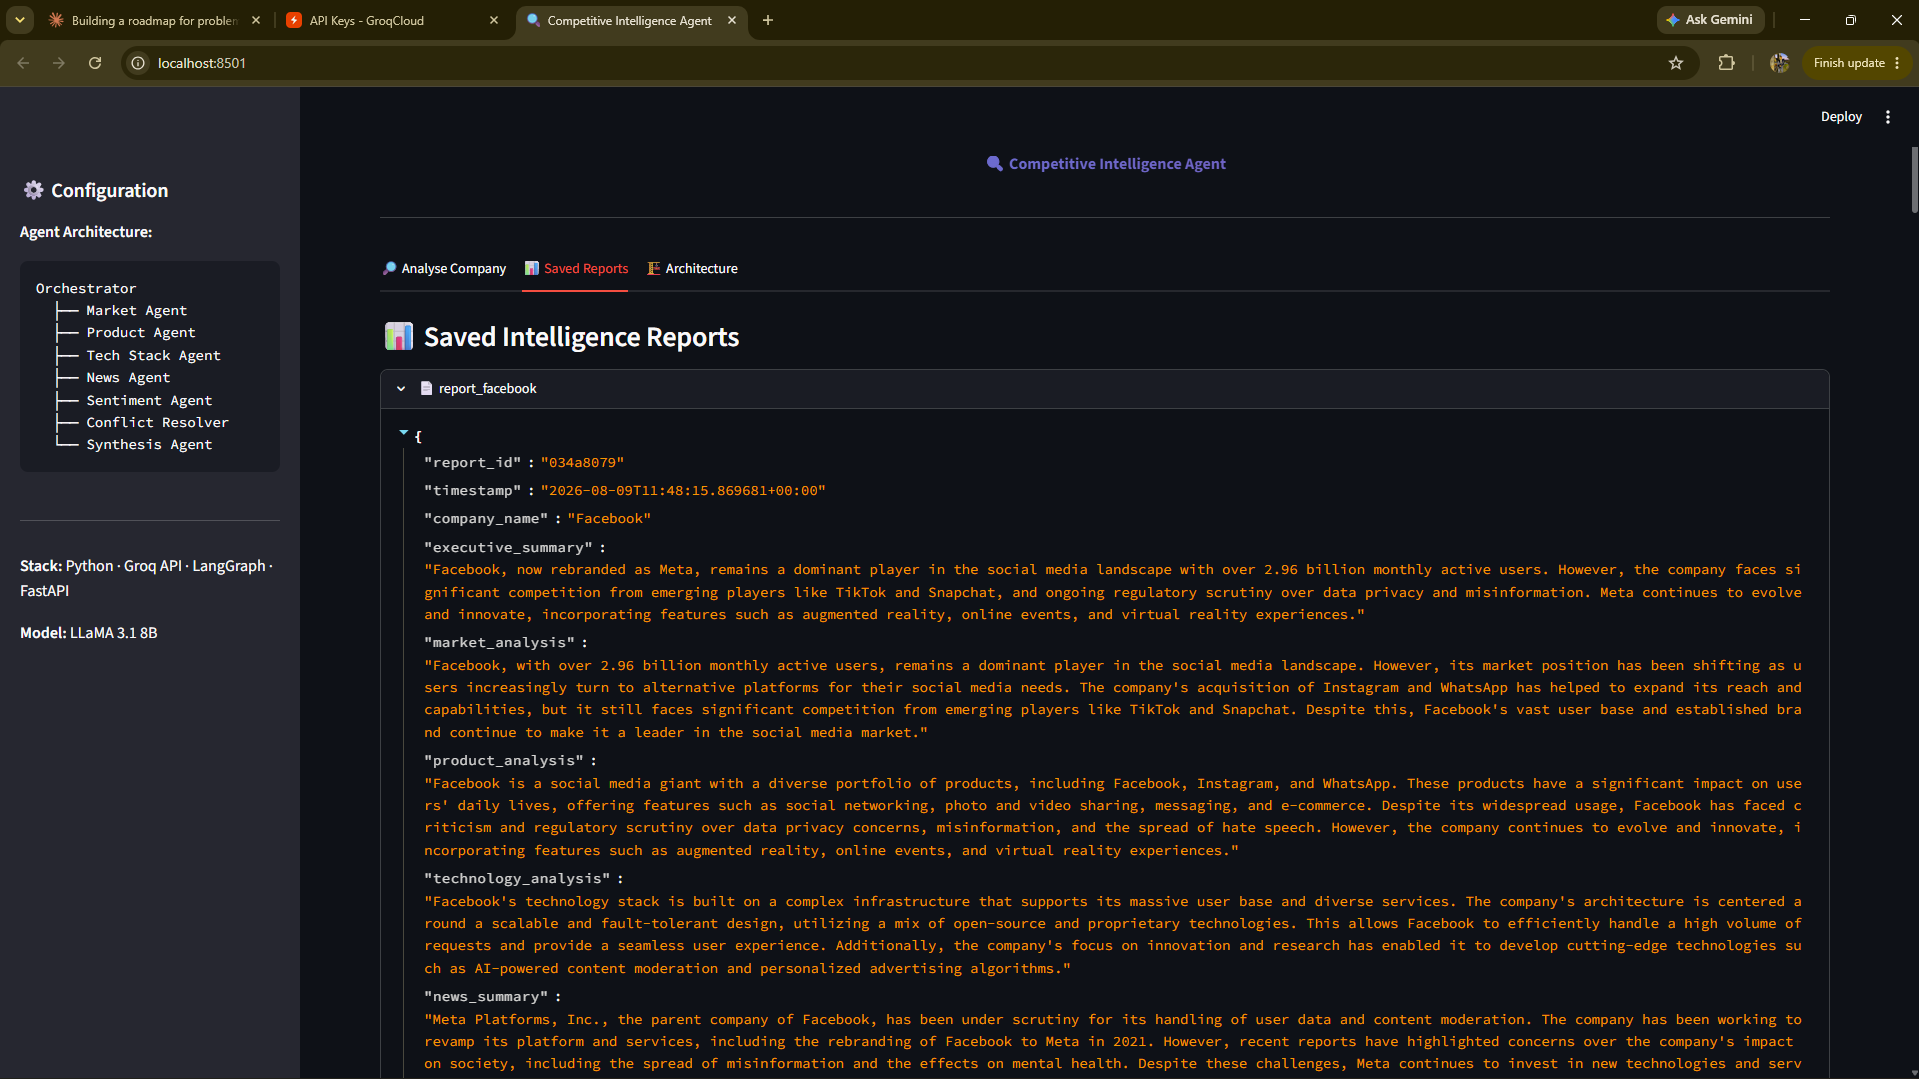
\includegraphics[width=\linewidth, keepaspectratio]{screenshots/Week5/Inter-3.png}
        \caption{Structured Findings Aggregation}
    \end{minipage}\hfill
    \begin{minipage}{0.48\textwidth}
        \centering
        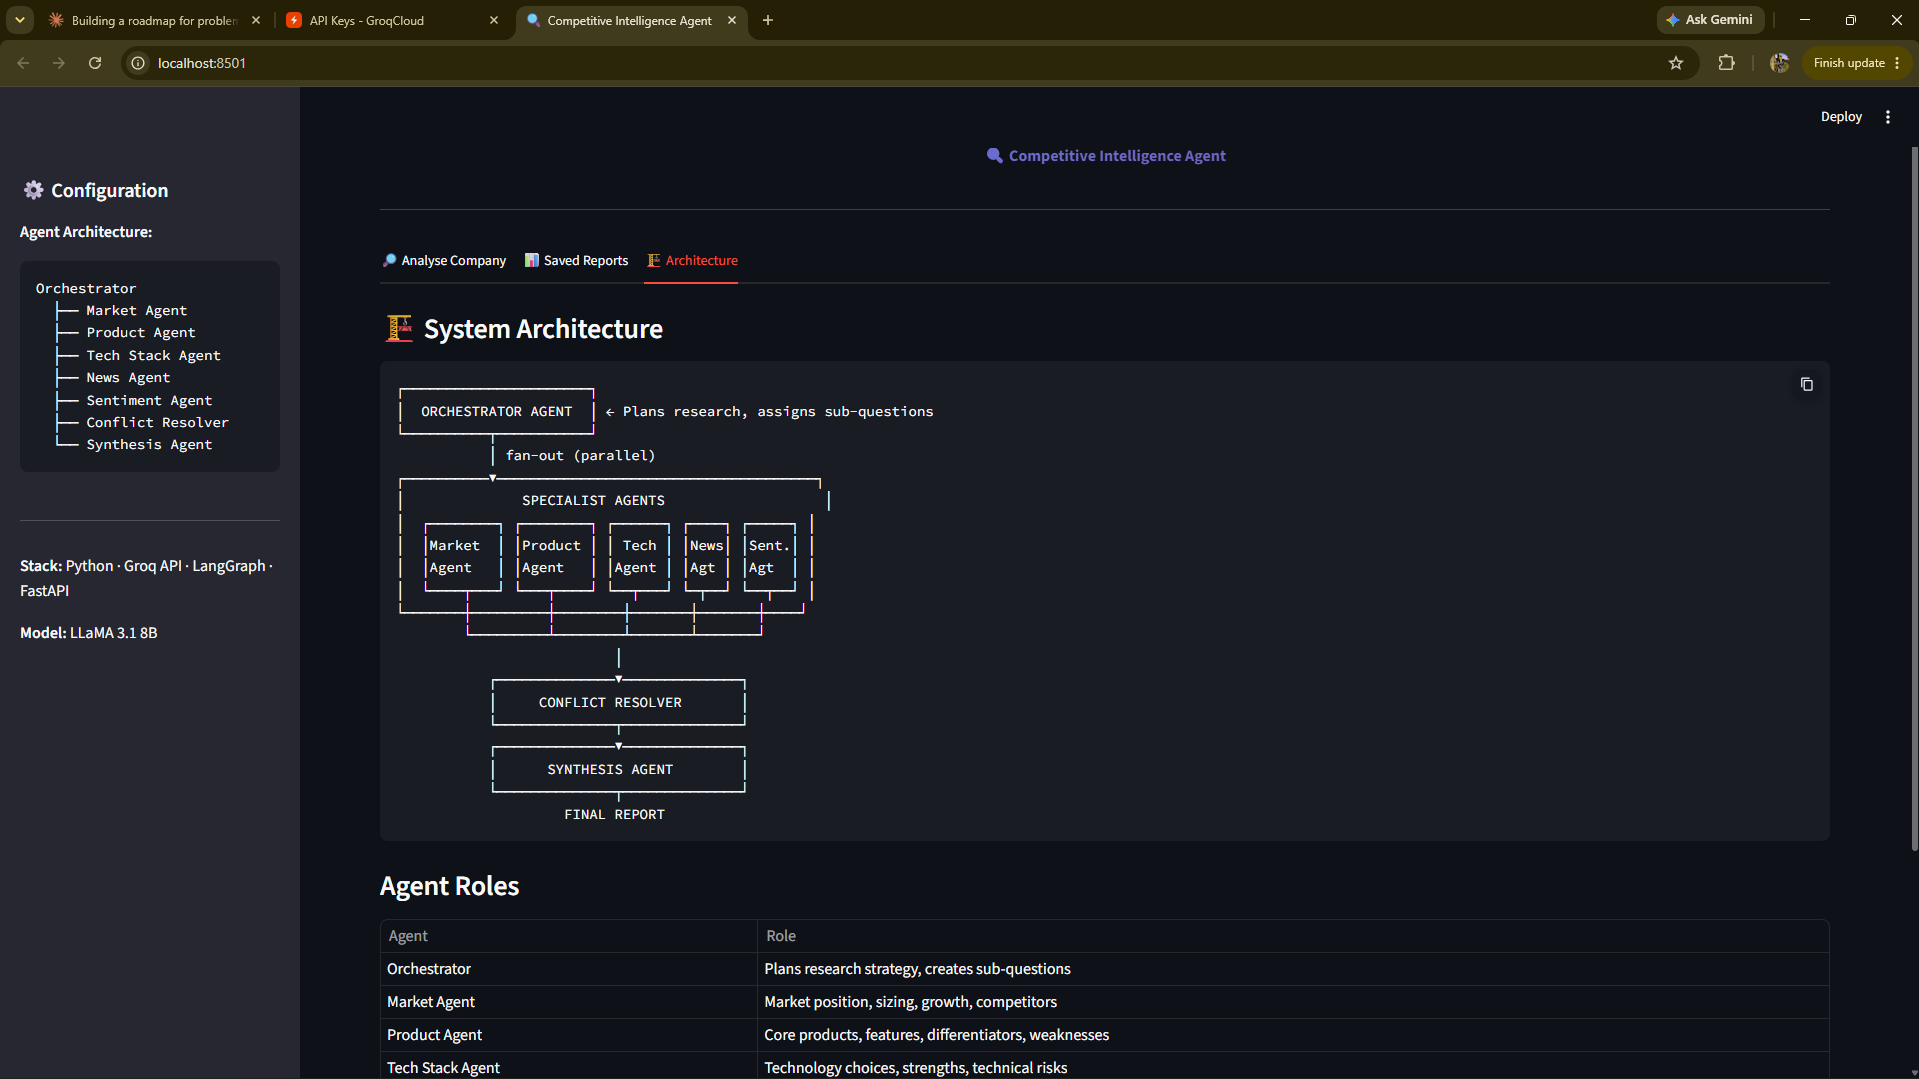
\includegraphics[width=\linewidth, keepaspectratio]{screenshots/Week5/Inter-4.png}
        \caption{System Architecture Representation}
    \end{minipage}
\end{figure}

\newpage

% --- Section 5: Foundational Labs ---
\section{Foundational Labs Deep-Dive}

\subsection{Lab 5.1: Typed Message Bus}
Developed the backbone for inter-agent communication by enforcing strict Pydantic message schemas over raw strings.
\begin{itemize}[label=\textcolor{secondary}{$\bullet$}]
    \item \textbf{Schema Validation:} Designed TaskRequest, TaskResult, ErrorReport, and Handoff models, ensuring malformed messages are caught by validation errors.
    \item \textbf{Reliable Handoffs:} Implemented three agents communicating exclusively over this in-memory typed message bus, guaranteeing type-safety.
\end{itemize}

\begin{figure}[H]
    \centering
    \begin{minipage}{0.48\textwidth}
        \centering
        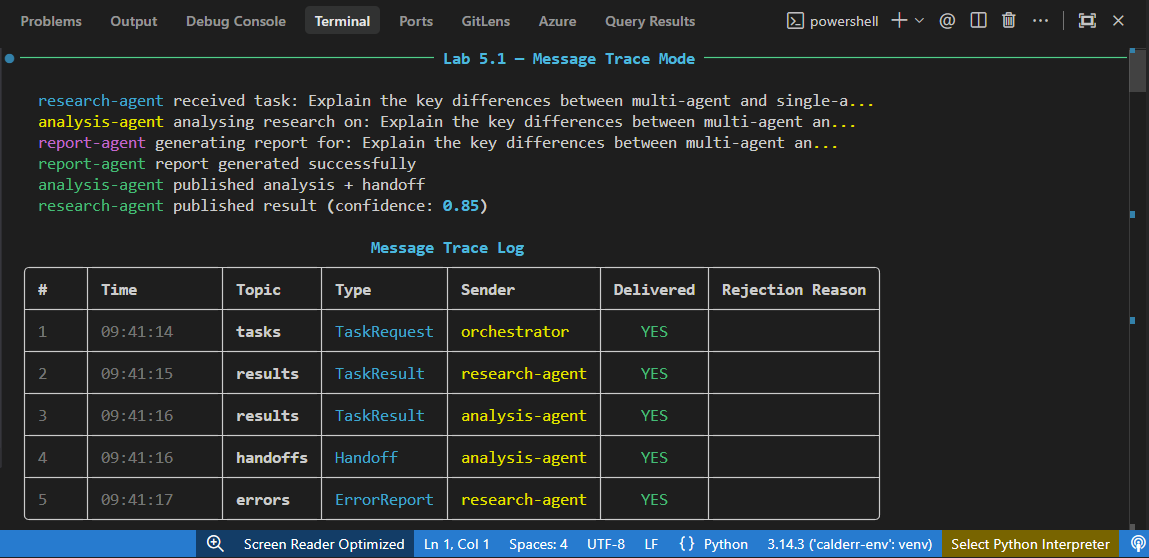
\includegraphics[width=\linewidth]{screenshots/Week5/Lab5.1-1.png}
        \caption{Typed Schema Validation}
    \end{minipage}\hfill
    \begin{minipage}{0.48\textwidth}
        \centering
        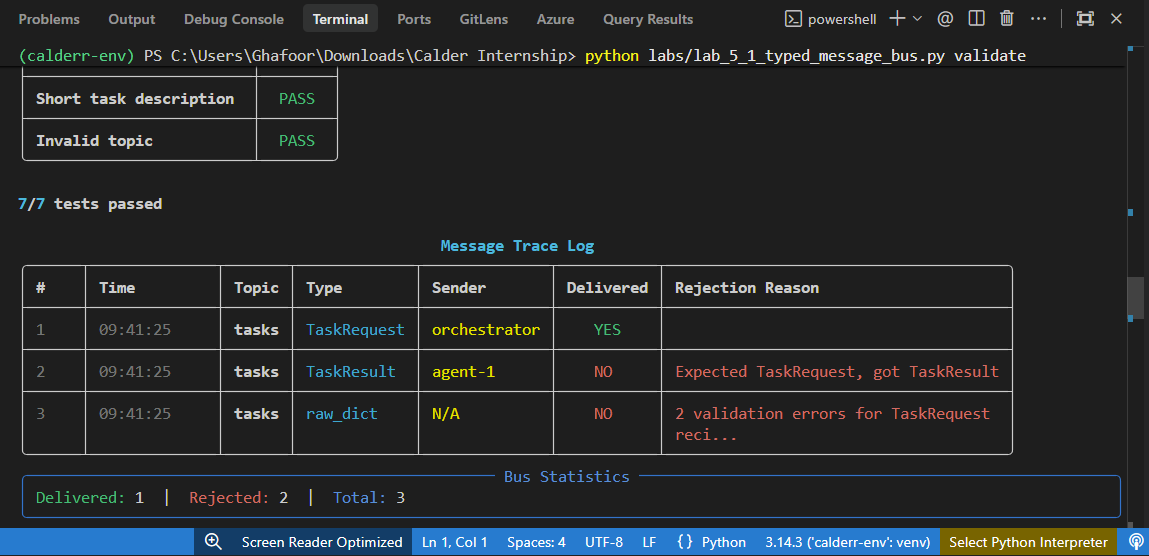
\includegraphics[width=\linewidth]{screenshots/Week5/Lab5.1-2.png}
        \caption{Agent Communication via Bus}
    \end{minipage}
\end{figure}
\begin{figure}[H]
    \centering
    \begin{minipage}{0.48\textwidth}
        \centering
        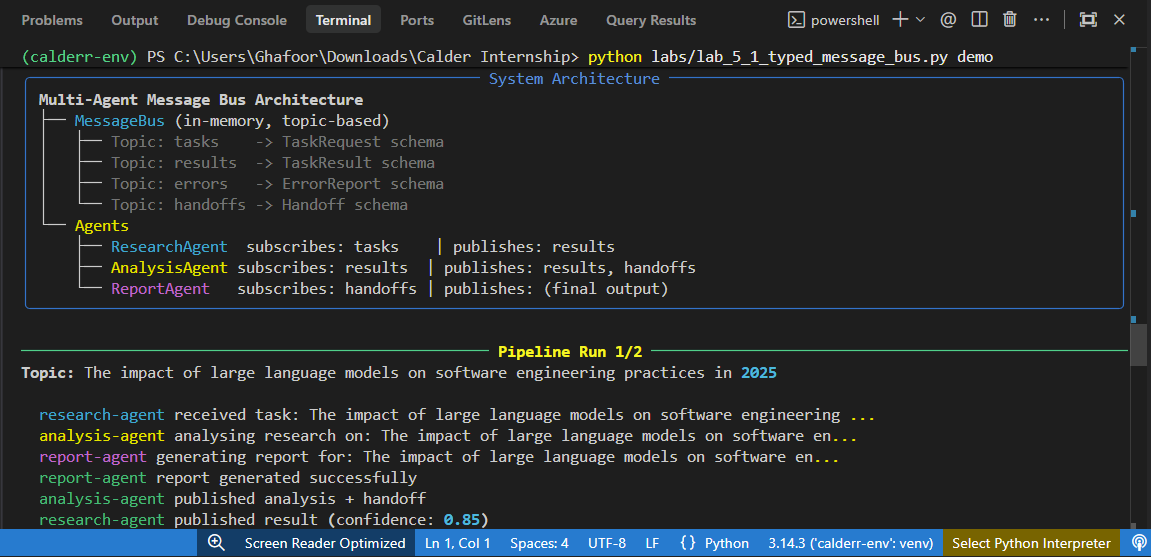
\includegraphics[width=\linewidth]{screenshots/Week5/Lab5.1-3.png}
        \caption{Handoff Execution}
    \end{minipage}\hfill
    \begin{minipage}{0.48\textwidth}
        \centering
        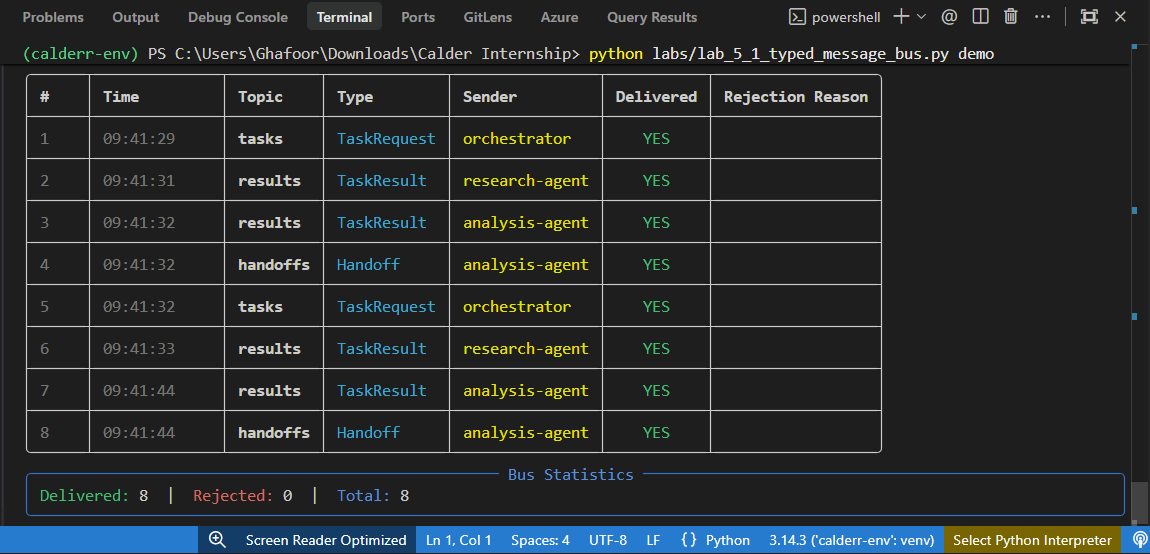
\includegraphics[width=\linewidth]{screenshots/Week5/Lab5.1-4.png}
        \caption{Error Handling in Messaging}
    \end{minipage}
\end{figure}

\vspace{0.5cm}

\subsection{Lab 5.2: Supervisor with Failure Recovery}
Built resilience into multi-agent systems by implementing a Supervisor Agent that gracefully manages routine failures from its delegate specialists.
\begin{itemize}[label=\textcolor{secondary}{$\bullet$}]
    \item \textbf{Fault Injection:} Tested the system against simulated timeouts and low-confidence responses.
    \item \textbf{Graceful Degradation:} Designed the supervisor to log failure reasons, route to fallback agents, and synthesize partial results to prevent system crashes.
\end{itemize}

\begin{figure}[H]
    \centering
    \begin{minipage}{0.31\textwidth}
        \centering
        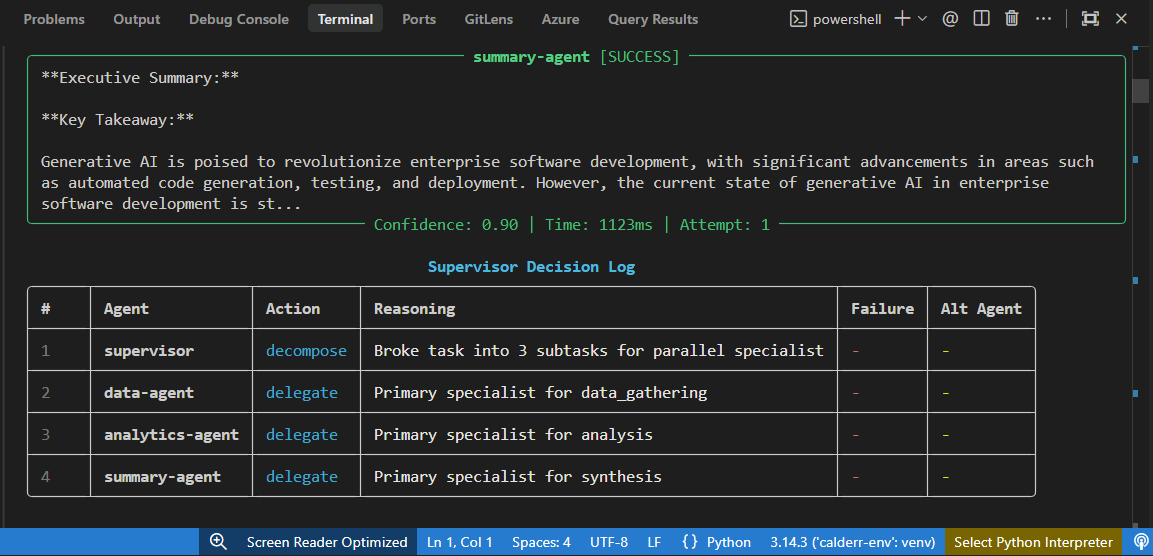
\includegraphics[width=\linewidth]{screenshots/Week5/Lab5.2-1.png}
        \caption{Delegation Trace}
    \end{minipage}\hfill
    \begin{minipage}{0.31\textwidth}
        \centering
        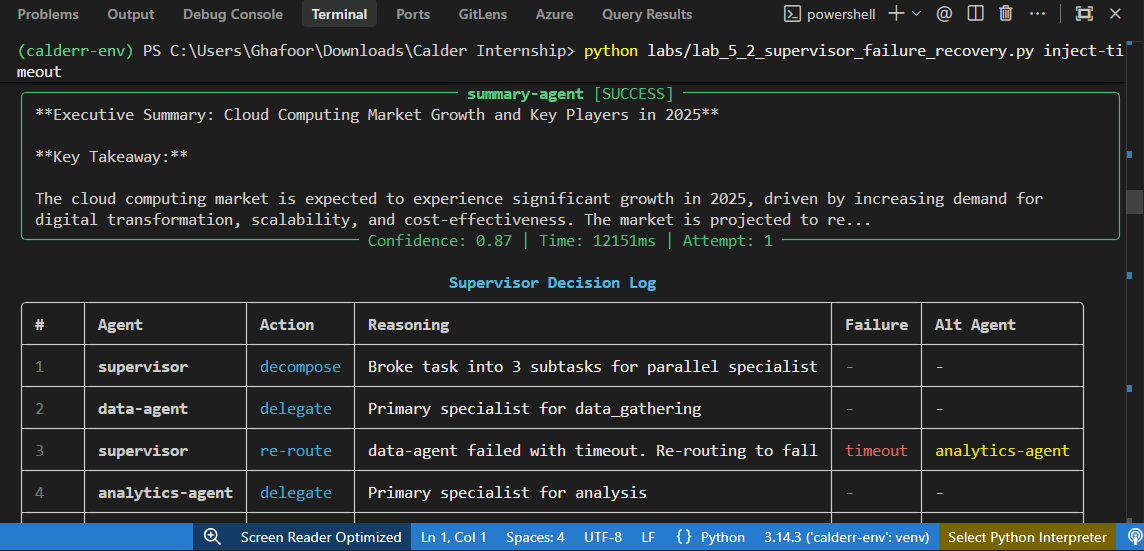
\includegraphics[width=\linewidth]{screenshots/Week5/Lab5.2-2.png}
        \caption{Timeout Detection}
    \end{minipage}\hfill
    \begin{minipage}{0.31\textwidth}
        \centering
        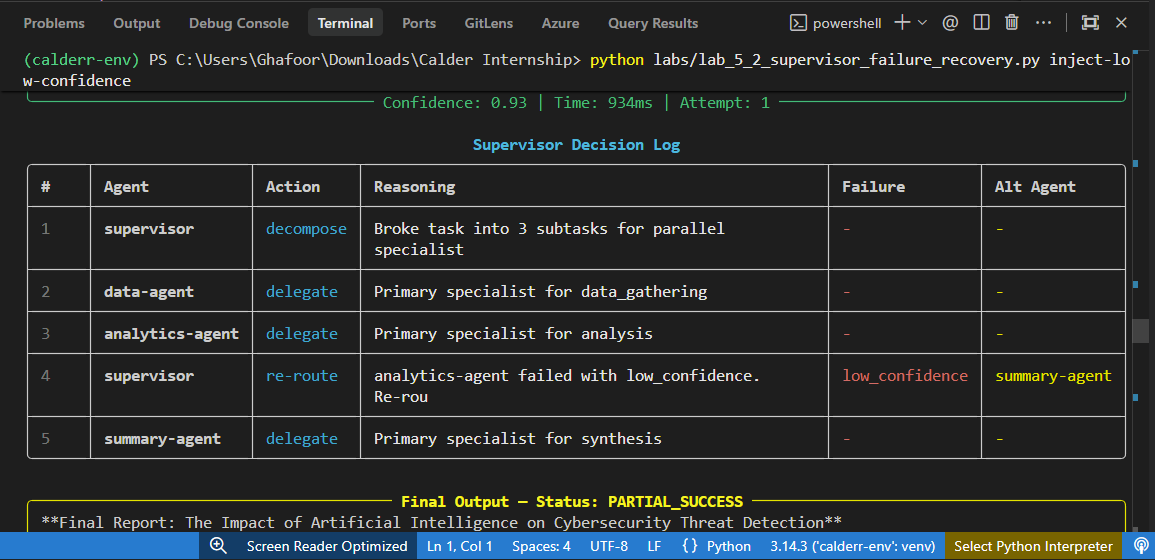
\includegraphics[width=\linewidth]{screenshots/Week5/Lab5.2-3.png}
        \caption{Fallback Routing Logic}
    \end{minipage}
\end{figure}
\begin{figure}[H]
    \centering
    \begin{minipage}{0.48\textwidth}
        \centering
        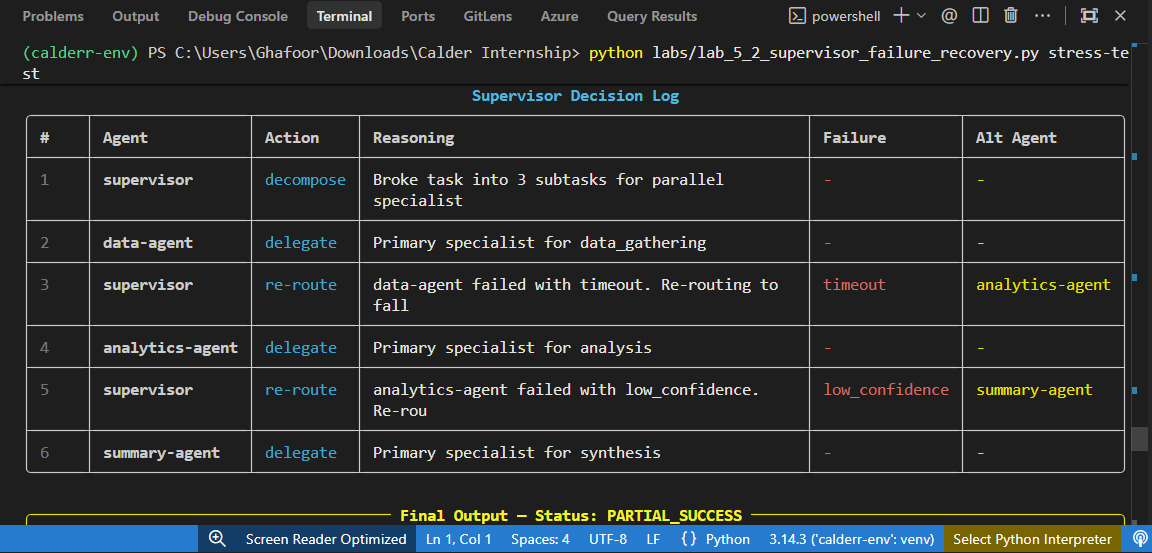
\includegraphics[width=\linewidth]{screenshots/Week5/Lab5.2-4.png}
        \caption{Supervisor Decision Log}
    \end{minipage}\hfill
    \begin{minipage}{0.48\textwidth}
        \centering
        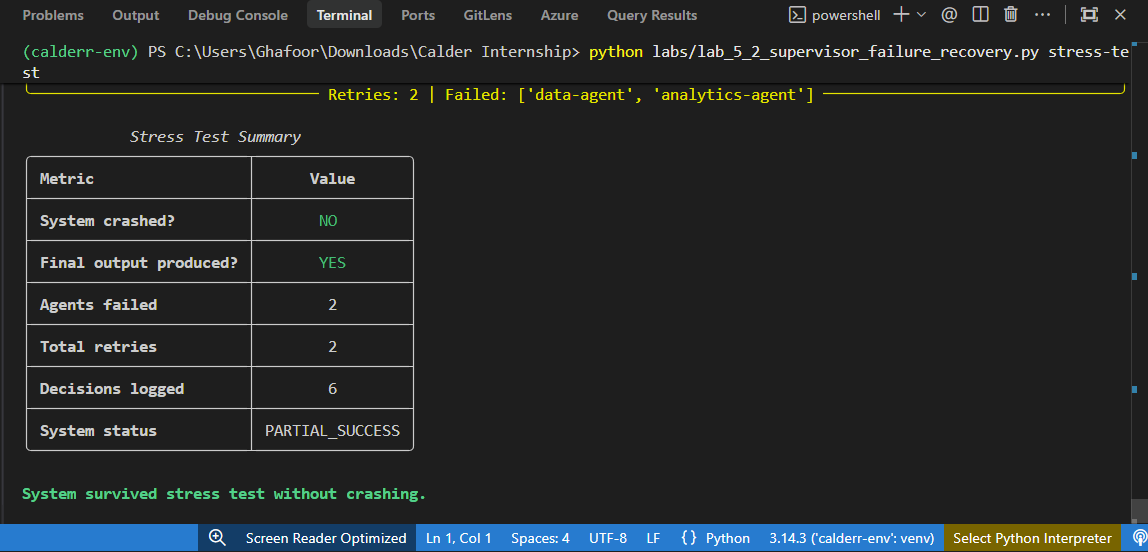
\includegraphics[width=\linewidth]{screenshots/Week5/Lab5.2-5.png}
        \caption{Gracefully Degraded Response}
    \end{minipage}
\end{figure}

\newpage

\subsection{Lab 5.3: Consensus Engine}
Engineered a debate and voting system to handle complex queries where multiple specialist agents form independent opinions.
\begin{itemize}[label=\textcolor{secondary}{$\bullet$}]
    \item \textbf{Confidence-Weighted Voting:} The Consensus Agent aggregates answers by multiplying opinions with confidence scores (0--1).
    \item \textbf{Multi-Round Debate:} Configured thresholds (60\%) that trigger a second debate round among the top 2 agents if consensus isn't reached, explicitly highlighting dissent in the final summary.
\end{itemize}

\begin{figure}[H]
    \centering
    \begin{minipage}{0.31\textwidth}
        \centering
        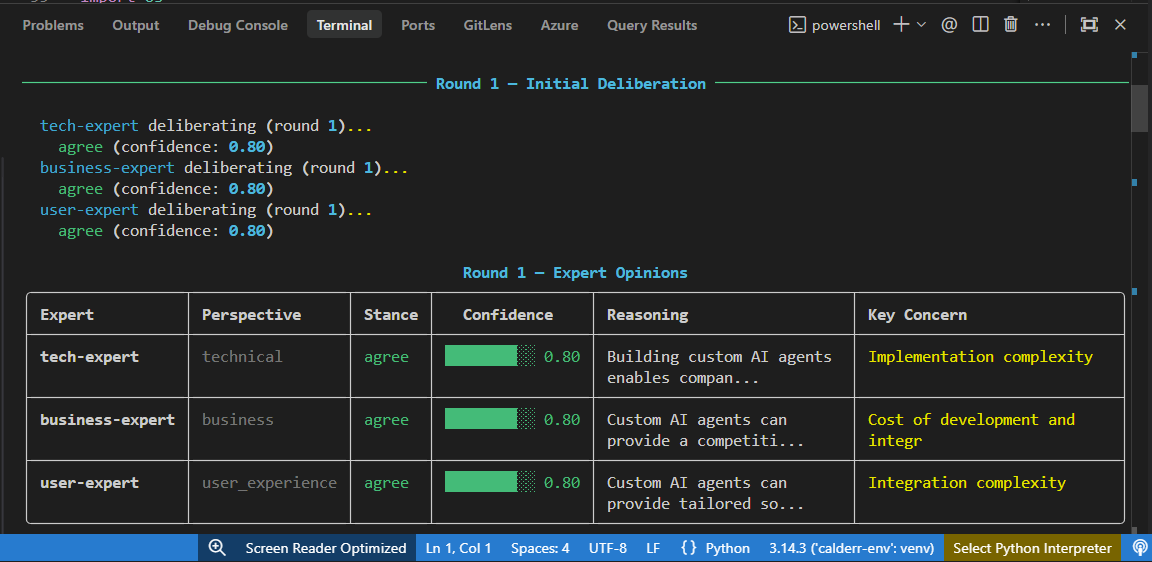
\includegraphics[width=\linewidth]{screenshots/Week5/Lab5.3-1.png}
        \caption{Initial Independent Opinions}
    \end{minipage}\hfill
    \begin{minipage}{0.31\textwidth}
        \centering
        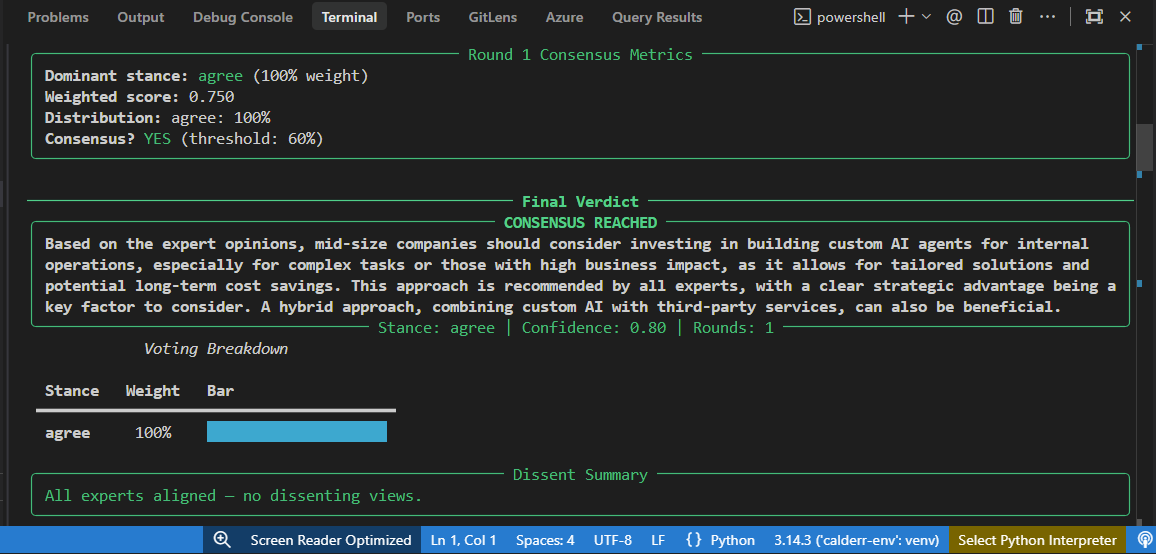
\includegraphics[width=\linewidth]{screenshots/Week5/Lab5.3-2.png}
        \caption{First Voting Round}
    \end{minipage}\hfill
    \begin{minipage}{0.31\textwidth}
        \centering
        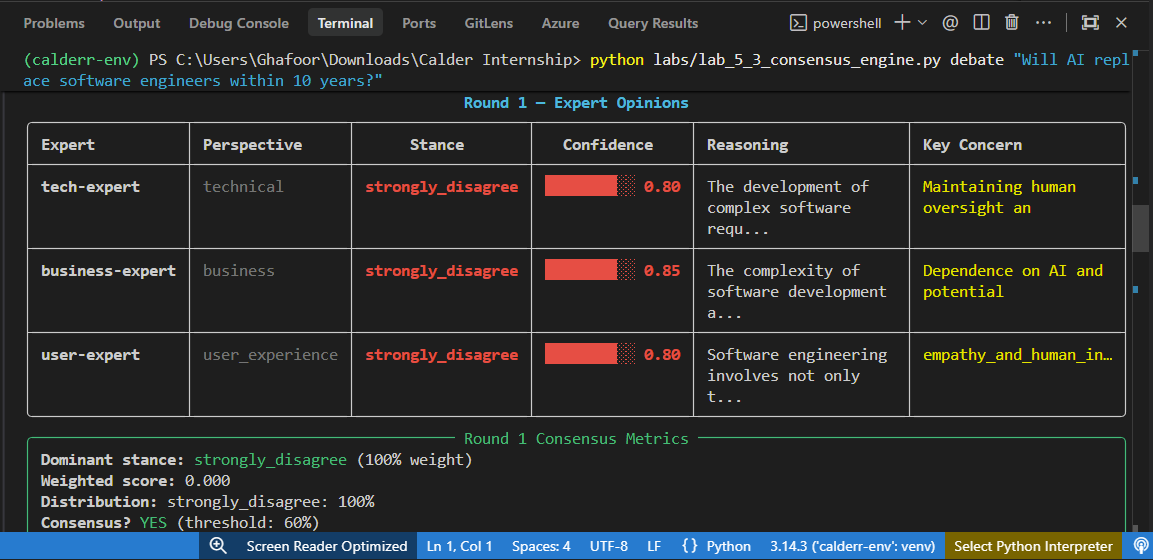
\includegraphics[width=\linewidth]{screenshots/Week5/Lab5.3-3.png}
        \caption{Triggering Round Two}
    \end{minipage}
\end{figure}
\begin{figure}[H]
    \centering
    \begin{minipage}{0.31\textwidth}
        \centering
        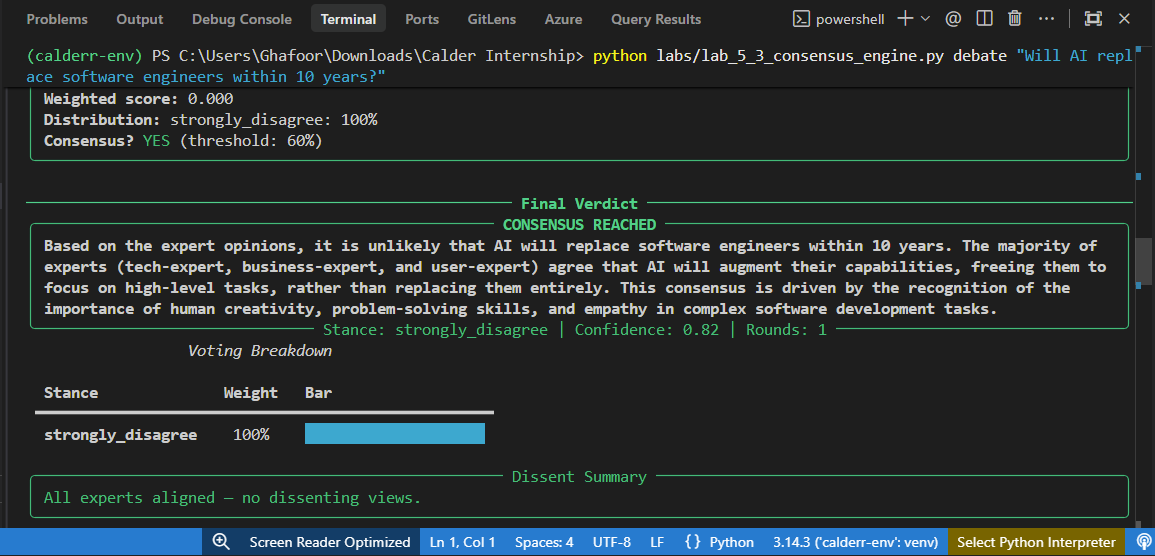
\includegraphics[width=\linewidth]{screenshots/Week5/Lab5.3-4.png}
        \caption{Second Round Debate}
    \end{minipage}\hfill
    \begin{minipage}{0.31\textwidth}
        \centering
        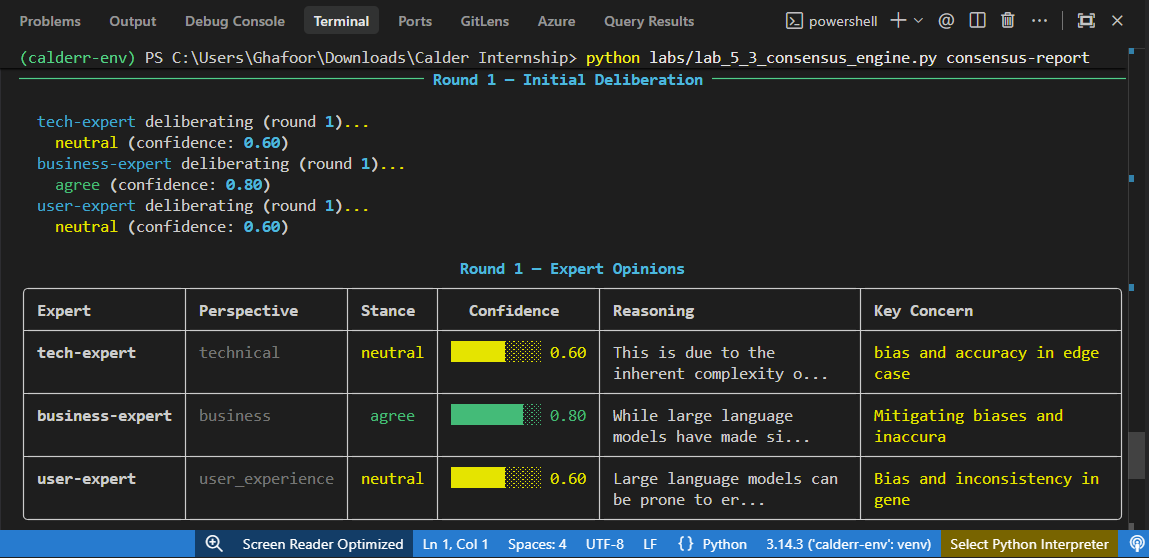
\includegraphics[width=\linewidth]{screenshots/Week5/Lab5.3-5.png}
        \caption{Consensus Aggregation}
    \end{minipage}\hfill
    \begin{minipage}{0.31\textwidth}
        \centering
        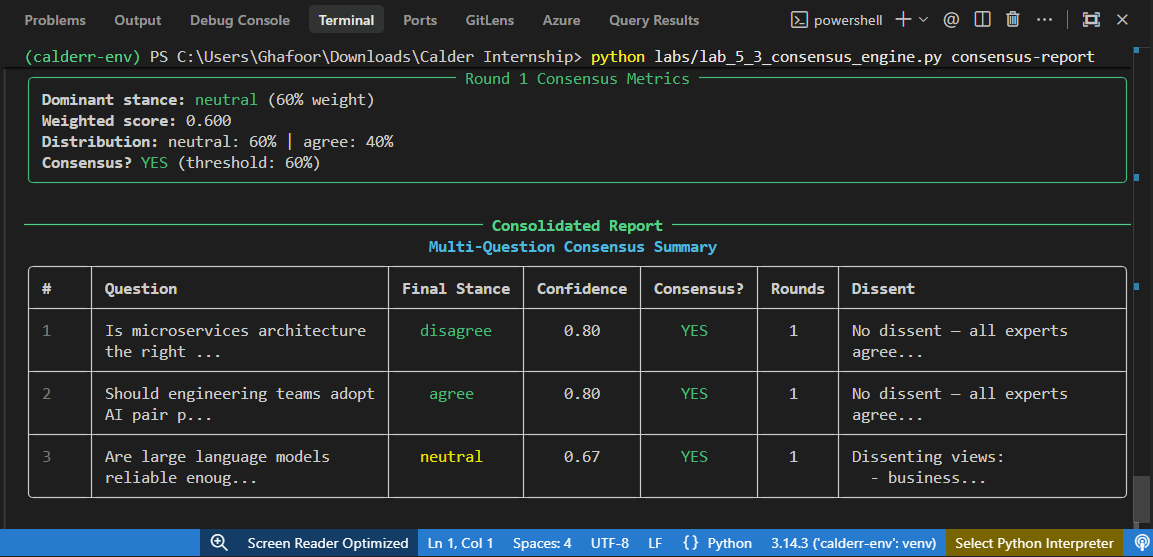
\includegraphics[width=\linewidth]{screenshots/Week5/Lab5.3-6.png}
        \caption{Final Output \& Dissent}
    \end{minipage}
\end{figure}

\vspace{0.5cm}

% --- Conclusion ---
\section{Conclusion \& Next Steps}
Week 5 represented a significant paradigm shift from engineering single agents to orchestrating complex, autonomous teams. By mastering graph-based delegation, enforcing typed communication, designing specialized personas, and implementing robust failure recovery and conflict adjudication, the projects developed this week mirror genuine production architectures. These advanced multi-agent patterns form the core capabilities required to solve sophisticated real-world engineering challenges autonomously.

\end{document}
